\documentclass{iaesarticle}

%%required package. add for your convenient, but do not remove the initial
\setlength{\headsep}{0.15in}
\usepackage{amsmath, amsfonts, amssymb, float, fancyhdr}
\usepackage[figuresright]{rotating}
\usepackage{authblk, graphicx, indentfirst, lastpage, lipsum}
\usepackage{pifont}
\renewcommand{\Authsep}{, }
\renewcommand{\Authand}{, }
\renewcommand{\Authands}{, }
\setlength{\affilsep}{0cm}
\renewcommand\Authfont{\normalsize}
\renewcommand\Affilfont{\fontsize{8}{10}\mdseries}
\makeatletter
\renewcommand{\@biblabel}[1]{[#1]\hfill}
\renewcommand\AB@authnote[1]{\textsuperscript{\normalfont\bfseries#1}}
\makeatother
\usepackage[font=normalsize]{subfig, caption}
\usepackage{epstopdf}
\usepackage[left=3cm, right=2.5cm, top=2.5cm, bottom=2.5cm, includehead, includefoot]{geometry}
\usepackage[justification=centering]{caption}
\captionsetup{labelsep=period}
\usepackage{titlesec}
\usepackage[table]{xcolor}
\titleformat{\section}
{\normalfont\normalsize\bfseries\uppercase}{\thesection}{1.7em}{}
\titleformat{\subsection}
{\normalfont\normalsize\bfseries}{\thesubsection}{.95em}{}
\titleformat{\subsubsection}
{\bfseries}{\thesubsubsection}{.2em}{}
\titlespacing*{\section}{0cm}{0.7cm}{0cm}
\usepackage{enumitem}
\usepackage[numbers,sort&compress]{natbib}
\usepackage{ragged2e}
\usepackage[hidelinks]{hyperref}
\usepackage{graphicx}
\usepackage{multirow}
\usepackage{tabularx}
\usepackage{booktabs}
\usepackage{fleqn}
\usepackage{tikz}
\usetikzlibrary{arrows.meta, shapes.geometric, positioning}

% --- Placeholder gambar sementara (hapus/ganti saat gambar asli tersedia) ---
% Pemakaian: \figplaceholder{lebar}{nama-berkas-gambar-nanti}
\newcommand{\figplaceholder}[2]{%
  \fbox{\parbox[c][3.2cm][c]{#1}{\centering\ttfamily\small [Gambar menyusul: #2]}}%
}

\CopyrightLine[]{}{\textit{This is an open access article under the \textcolor{blue}{\underline{CC BY-SA}} license.}
\vspace{.5em}}

%%author
\author[1]{\bfseries Hero Yudo Martono}
\author[2]{\bfseries Nafisah Rahmadani Harahap}
\author[3]{\bfseries Iwan Syarif}
\author[4]{\bfseries Ferry Astika Saputra}

%%author's affiliation
\affil[1,2,3,4]{Department of Informatics Engineering, Politeknik Elektronika Negeri Surabaya, Surabaya, Indonesia}

%%title and shortitle (for footer)
\title{Design of a cloud backup system based on multi-compression algorithms for ransomware attack mitigation}
\shorttitle{Design of a cloud backup system based on multi-compression algorithms ... (Martono)}

%%starting
\begin{document}
\setcounter{page}{1}

%%indentation. do not change
\setlength{\parindent}{1.27cm}

%%header and footer setting. do not change
\pagestyle{fancy}
\fancyhfoffset{0cm}

%%journal info
\journalname{International Journal of Electrical and Computer Engineering (IJECE)}
\journalshortname{Int J Elec \& Comp Eng}
\journalhomepage{http://ijece.iaescore.com}
\vol{99}
\no{1}
\months{Month}
\years{2099}
\issn{2088-8708}
\DOI{10.11591}
\pagefirst{1}
\pagelast{1x}
\IDpaper{42551}

%%build title
\maketitle

%%border setting. do not change
\hrule
\vspace{.1em}
\hrule
\vspace{.5em}
\noindent
\parbox[t][][s]{0.315\textwidth}{%
\textbf{Article Info}
\vspace{.5em}
\hrule
\vspace{.5em}
\begin{history}
\vspace{.5em}
Received month dd, yyyy

Revised month dd, yyyy

Accepted month dd, yyyy

\vspace{.7em}
\end{history}
\vspace{.5em}
\hrule
\vspace{.5em}
\begin{keyword}
\vspace{.5em}
Cloud backup and restore \sep
Ransomware resilience \sep
Air gapped backup \sep
Lossless compression \sep
Anomaly detection
\vspace{.5em}
\end{keyword}
\vspace{\fill}
}
\parbox{0.020\textwidth}{\hspace{0.5em}}
\parbox[t][][s]{0.65\textwidth}{%
\begin{abstract}
\vspace{.3em}
Ransomware has become one of the most damaging threats to data availability and integrity in cloud storage environments. The problem is that conventional backup systems still leave a gap: their backup repositories are often directly reachable from the primary system, so they become infected when an attack occurs. On the other hand, using a single compression algorithm for all files is rarely efficient because the file types handled are highly heterogeneous. This study addresses both problems through a cloud backup system that combines an \textit{air-gapped} mechanism with adaptively selected multi-algorithm \textit{lossless} compression. To distinguish legitimate backup encryption from ransomware-induced file corruption, the system inspects three indicators at once: the SHA-256 \textit{hash} value, metadata, and file structure. Evaluation was performed in a controlled manner using a simulated attack model---without executing real \textit{malware}---on a limited synthetic \textit{dataset} of 43 files with varying types and sizes, under both normal and attacked conditions. For low-entropy text files, compression reduced storage by up to 89.5\% (log) and 81.1\% (CSV) using Brotli; Snappy and LZ4 yielded 66--80\% savings but far faster. Conversely, already-compressed JPG and XLSX files barely shrank. When attacked, the system recovered all 43 files without a single error within 4.3--5.3 seconds, with a \textit{False Positive Rate} (FPR) and \textit{False Negative Rate} (FNR) both at 0\% in the controlled test environment. These findings show that combining \textit{air-gapped} isolation, adaptive compression, and integrity verification can strengthen both the security and the storage efficiency of cloud backups against ransomware.
\end{abstract}
}
\parbox[l]{\textwidth}{%
\rule{0.275\textwidth}{0.5pt} \hspace{0.5cm} \hrulefill
\\
\emph{\textbf{Corresponding Author:}}
\vspace{.5em}\\
Hero Yudo Martono\\
Department of Informatics Engineering, Politeknik Elektronika Negeri Surabaya\\
Surabaya, Indonesia\\
Email: hero@pens.ac.id
}
\vspace{.5em}
\hrule
\vspace{.1em}
\hrule

%% main text
\section{Introduction}
\label{sec:introduction}
Over the past decade, digital technology has advanced rapidly and reshaped many sectors---finance being among the most affected. Digitalization in this field is no longer limited to processing transactions; it now extends to data recording, reporting, risk monitoring, and real-time analytics \cite{1}, \cite{2}. As a consequence, the volume of data to be managed has swelled, demanding large-scale storage that is both secure and efficient amid ever-growing cyber threats \cite{3}, \cite{4}. This accumulating data takes many forms: daily transaction records, system logs, user data, financial reports, and audit documents \cite{5}. A single financial institution may process millions of transactions per day and generate hundreds of gigabytes to terabytes of data that must be archived for operational, audit, and regulatory-compliance purposes. It is precisely this need that calls for a storage system that is not only secure and economical but also underpinned by backup mechanisms that keep data available and intact.

Among the various cyber threats, ransomware occupies the most alarming position for today's organizations. This type of \textit{malware} locks victims' data through encryption and then demands a ransom as the condition for restoring access \cite{5}, \cite{6}. What makes it increasingly dangerous is that modern variants do not stop at production systems---backup infrastructures still connected to the network are targeted as well \cite{7}, \cite{8}. Once backups become infected, the chance of recovering critical data vanishes, and the organization suffers operational disruption, financial loss, and reputational damage \cite{9}. The Sophos \textit{State of Ransomware in Financial Services 2024} report even records that about 43\% of devices in financial organizations have been affected by such incidents. This reality underscores that conventional backups, permanently connected to the network, can no longer be relied upon. One proven answer is the \textit{air-gapped} backup architecture, which isolates backup storage---physically or logically---from the primary network so that ransomware has no direct path to it \cite{10}. Unfortunately, building a fully physical \textit{air-gap} tends to be costly and operationally complex, especially for small and medium-sized organizations in developing countries. For that reason, this study takes the logical \textit{air-gapped} route: using controlled \textit{mounting} and isolated backup media so that ransomware resilience is still achieved without burdening cost and operations. The proposed design deliberately prioritizes affordability, ease of deployment, and compatibility with the cloud infrastructures commonly used by local organizations and financial institutions.

In recent years, the scale of this threat has surged sharply. A survey synthesizing more than 50 research articles over 2020--2025 records that global ransomware losses exceeded USD 30 billion in 2023---about a 900\% rise from 2015---with more than 493 million attacks detected in 2022, an average ransom of USD 2.73 million in 2024, and operational disruption lasting 21 days on average \cite{41}. Recent reviews add an important note: ransomware has now entered the era of \textit{data exfiltration}, while most academic research still lags behind real-world attack patterns \cite{23}, \cite{26}. Its form has changed too, from mere screen-locking into layered attack chains employing \textit{double} or even \textit{triple extortion}---encrypting data, leaking it, then launching DDoS. The situation is further complicated by the \textit{Ransomware-as-a-Service} (RaaS) model on the \textit{darknet} \cite{40} and shifting tactics documented throughout the pandemic period \cite{33}. All of this indicates that defending solely by preventing infection is no longer adequate \cite{42}, \cite{46}. To organize the diverse defense approaches, the literature offers the \textit{Detection--Avoidance--Mitigation} (DAM) framework, which divides them into three stages: detection (static, dynamic, and hybrid analysis), avoidance (security awareness and \textit{hardening}), and mitigation (backup and recovery) \cite{42}. Within this map, our study occupies the \textbf{mitigation and recovery} stage: ensuring data remains available and recoverable even when early detection fails, rather than competing on \textit{machine learning}-based detection accuracy.

The problem does not end with security. The ever-growing volume of archival data makes storage efficiency equally important. For rarely accessed data---transaction logs, audit records, system backups---many organizations turn to cold cloud storage because of its lower cost \cite{11}. Even so, storing large-scale backups in the cloud still demands careful space optimization and bandwidth management. This is where \textit{lossless} compression plays a role: trimming storage needs without sacrificing data integrity \cite{12}, \cite{13}. The issue is that previous research has tended to treat backup security, ransomware mitigation, or compression as standalone topics, so few have combined a secure backup architecture with adaptive storage optimization \cite{14}, \cite{15}. Existing systems also generally rely on a single static compression algorithm, even though files of different types and sizes present non-uniform compression characteristics and performance trade-offs \cite{16}, \cite{17}.

The link between compression efficiency and security actually stems from a single data property: \textit{entropy}. Shannon's information theory states that the \textit{lossless} compression limit of a file is determined by its entropy, $H(X) = -\sum_{i} p(x_i)\log_2 p(x_i)$, namely the average minimum number of bits needed to represent each symbol. Low-entropy files---\textit{plaintext} such as CSV and logs full of repeated patterns---contain much redundancy and can therefore be compacted freely. Conversely, high-entropy files such as encrypted data or already-compressed JPGs are nearly random, so they can hardly be reduced further. This property gives rise to two interrelated consequences. First, to be efficient, the choice of compression algorithm should adapt to the entropy or type of the file. Second, a sudden entropy spike in a file that was originally low can signal illegitimate encryption by ransomware. Unfortunately, entropy-based detection has a weak spot: \textit{Format-Preserving Encryption} (FPE) preserves file structure so that entropy does not spike noticeably and the detector can be fooled. This gap is the \textit{research gap} of our study---no framework yet unites (a) storage optimization through adaptive compression based on file characteristics, (b) ransomware-resilient backup isolation, and (c) integrity verification that does not rely on entropy alone but on \textit{hash} and metadata---within a single cloud backup system.

Instead of relying on static compression or separate backup protection as most prior research does, this study offers an integrated cloud backup system---combining an \textit{air-gapped} storage architecture with an adaptive multi-compression framework. The system dynamically selects among five \textit{lossless} algorithms, namely Gzip, Zstandard, Brotli, LZ4, and Snappy, through a rule-based selection that considers file characteristics such as size and data type, in order to balance compression ratio, speed, and resource usage. What sets it apart is that this study embeds multi-indicator anomaly detection---a combination of SHA-256 \textit{hash} analysis, metadata validation, and file structure inspection---to separate ransomware encryption patterns from legitimate AES-256 encryption within the backup environment. This capability closes a weakness that frequently appears in earlier studies, which tend to treat all encrypted files the same without separating malicious encryption from authorized security encryption.

Accordingly, the contribution of this study lies in an integrated approach that simultaneously addresses ransomware resilience, backup isolation, adaptive compression efficiency, and integrity verification within a single cloud backup framework. This combination of \textit{air-gapped} architecture, adaptive multi-algorithm compression, AES-256 encryption, SHA-256 integrity verification, and multi-indicator anomaly detection is designed to strengthen backup security along with long-term storage efficiency for cloud-based financial data infrastructures \cite{18}, \cite{19}, \cite{20}.

\section{Related Work}
\label{sec:related_work}
Several previous studies have addressed cloud-based backup systems, data compression techniques, and ransomware mitigation methods. However, most studies focus only on a single aspect independently, such as compression performance, storage efficiency, or backup security, without integrating these components into a unified system. In addition, previous works rarely discuss the fundamental distinction between air-gapped and conventional connected (non-air-gapped) backup architectures in ransomware mitigation scenarios. A comparison of related studies and the proposed system is presented in Table~\ref{tab:related_work}.

\begin{table}[H]
\centering
\fontsize{8pt}{10pt}\selectfont
\caption{Related work}
\label{tab:related_work}
\begin{tabularx}{\textwidth}{@{}c p{2.2cm} X X X X@{}}
\hline
\textbf{No} & \textbf{Study} & \textbf{Research Focus} & \textbf{Methods} & \textbf{Limitations} & \textbf{Contribution of this study} \\
\hline
1 & M. Smith and Lee, Data in Brief 2023 & Performance evaluation of compression algorithms & Gzip, Zstd, Brotli, LZ4, Snappy & Does not address backup security & Integrates compression with backup systems \\
2 & S. Kumar and R. Patel, 2024 & Data compression in cloud-based e-commerce & Brotli, Snappy, Gzip & Focuses only on data transfer performance & Applied within backup systems for storage efficiency \\
3 & A. Novak, P. Chen, and R. Singh (2021) & Backup system for ransomware mitigation & Hybrid compression + air-gapped & Focus limited to the financial sector & Implementation of cloud backup with anomaly detection mechanisms \\
4 & S. Kumar and R. Patel, IEEE Access, 2022 & Optimization of cloud backup against ransomware & Zstd, LZ4, Gzip & Does not provide a comprehensive comparison of multiple algorithms & Evaluation of multiple compression algorithms \\
5 & M. Sahu and J. Panda, arXiv & Compression study & Snappy, Gzip, BZIP2 & Limited analysis on efficiency aspects & Integration of storage efficiency and security \\
6 & NIST (2024) Air-Gapped Backup Guideline & Secure offline backup for ransomware protection & Physical/logical air-gapped storage & Does not optimize storage efficiency, lacks compression & Combines air-gapped backup with adaptive multi-compression and anomaly detection \\
\hline
\end{tabularx}
\end{table}

Previous studies generally focused on compression performance or backup security in isolation. Smith and Lee evaluated several compression algorithms but did not address ransomware protection. Kumar and Patel focused on storage optimization and cloud backup efficiency but lacked anomaly detection and automated recovery mechanisms. Meanwhile, Novak et al. introduced an \textit{air-gapped} backup system for ransomware mitigation; however, its implementation remained limited and did not comprehensively evaluate storage efficiency.

Based on these limitations, the novelty of the proposed study lies in integrating \textit{air-gapped} backup protection, adaptive multi-algorithm \textit{lossless} compression, and anomaly detection using \textit{hash} and metadata verification within a single cloud-based backup architecture. This integration improves ransomware resilience, storage efficiency, automated recovery capability, and practical deployment feasibility for enterprise-scale cloud backup environments.

The position of this study among the mainstream of ransomware detection research must be made clear so that its contribution is evident. Most recent studies focus on machine-learning-based \textit{detection}: classical \textit{machine learning} approaches for ransomware classification are reported to achieve high accuracy with feature selection \cite{31}, \textit{deep learning} models (CNN, LSTM, and CNN--LSTM hybrids) reach 96--99\% on balanced \textit{datasets} \cite{30}, and hardware-assisted detection approaches leverage \textit{automated machine learning} to improve robustness \cite{34}. Real-time detection systems that monitor encryption instructions (AES-NI) on the CPU can even halt an attack after only 10--15 files have been encrypted \cite{32}. However, all of these detection approaches face challenges consistently reported in the literature: the limitations of outdated \textit{datasets}, the difficulty of cross-platform detection, and the emergence of sophisticated evasion techniques such as \textit{Format-Preserving Encryption} (FPE) that fools entropy-based detection \cite{43}, \textit{fileless} attacks, and \textit{Living-off-the-Land} \cite{35}. Unlike that mainstream, this study \textbf{does not compete on detection accuracy}; rather, it strengthens the \textit{mitigation/recovery} layer---aligned with the body of work on backup strategies (the 3-2-1 rule, \textit{immutable}/WORM, \textit{air-gapped}) that reports high recovery rates without paying a ransom \cite{44}, and supported by structured ransomware incident-response frameworks \cite{45}. The proposed system is therefore complementary to ML-based detectors: when early detection fails, integrity mechanisms and isolated recovery guarantee data availability.

\begin{table}[H]
\centering
\fontsize{8pt}{10pt}\selectfont
\caption{Conceptual comparison of air-gapped and non air-gapped backup systems}
\label{tab:airgap_comparison}
\begin{tabularx}{\textwidth}{@{}p{3.2cm} X X@{}}
\hline
\textbf{Aspect} & \textbf{Air-Gapped Backup} & \textbf{Non Air-Gapped Backup} \\
\hline
Network connectivity & Isolated (physical or logical) & Connected to primary system \\
Ransomware resistance & High & Low \\
Risk of backup infection & Minimal & Potentially compromised \\
Data integrity & Preserved & Uncertain / failed \\
Recovery capability & Reliable & Uncertain / failed \\
Security level & Very high & Moderate \\
Compression strategy & Adaptive multi-algorithm & Single static compression \\
Storage efficiency & Up to 70--80\% reduction & Moderate \\
\hline
\end{tabularx}
\end{table}

As shown in Table~\ref{tab:airgap_comparison}, air-gapped backup systems provide stronger ransomware protection because the backup storage is isolated from the primary network. However, previous studies have not fully integrated this approach with storage optimization and anomaly detection mechanisms, which motivates the proposed system in this study. In practical deployment environments, many small and medium-sized organizations in Indonesia still rely on conventional connected cloud backup systems or default hosting backup solutions that utilize single-algorithm compression and continuously connected storage repositories. While these approaches provide operational simplicity, they remain vulnerable to ransomware propagation because backup repositories are directly accessible from compromised systems.

Compared with conventional backup approaches, the proposed system provides additional protection through logical air-gapped isolation, automated integrity verification, adaptive multi-algorithm compression, and ransomware-aware recovery mechanisms. Experimental results demonstrate that the proposed system achieved up to 70--80\% storage reduction for large structured datasets while maintaining 100\% successful recovery during ransomware simulation scenarios.

\section{Method}
\label{sec:method}
This study employs a quantitative experimental design to evaluate the performance of a cloud-based backup system integrating multiple \textit{lossless} compression algorithms \cite{22}, \cite{24}, \cite{25}. Each algorithm is tested independently in a single-mode configuration with evaluation parameters including storage efficiency, processing time, and resilience against simulated ransomware attacks. The proposed system adopts a hybrid \textit{air-gapped} backup architecture that combines offline local storage and cloud storage \cite{21}, \cite{27}. The experimental environment is designed to resemble real-world financial information systems, characterized by large-scale data storage requirements and long-term retention, while also incorporating ransomware detection and mitigation aspects as discussed in previous studies \cite{28}, \cite{29}.

\subsection{System architecture}
The proposed system architecture is organized into three logical layers that support the backup, compression, and detection processes. At the application layer, the system manages file upload, backup, and restore operations. Each incoming file undergoes cryptographic \textit{hash} computation using the SHA-256 algorithm, metadata extraction, and file structure analysis to establish an integrity baseline. This information is stored as a reference to detect future file changes and to distinguish legitimate modifications (e.g., backup or normal encryption) from malicious alterations caused by ransomware activity.

At the protection and compression layer, the system performs an initial metadata inspection to detect potential anomalies. Each file is then \textbf{compressed first} using one of five \textit{lossless} compression algorithms (Gzip, Zstandard, Brotli, LZ4, or Snappy), \textbf{and only then encrypted} with AES-256. This \textit{compress-then-encrypt} order matters technically: encrypted data has high entropy (close to randomness) and therefore cannot be compressed effectively; by compressing the \textit{plaintext} first, genuine storage savings can be obtained before the confidentiality layer is applied \cite{9}. Each algorithm is applied independently to the same dataset to obtain empirical measurements, including compression ratio and processing time, enabling a consistent performance comparison \cite{10}, \cite{36}.

\begin{figure}[H]
\centering
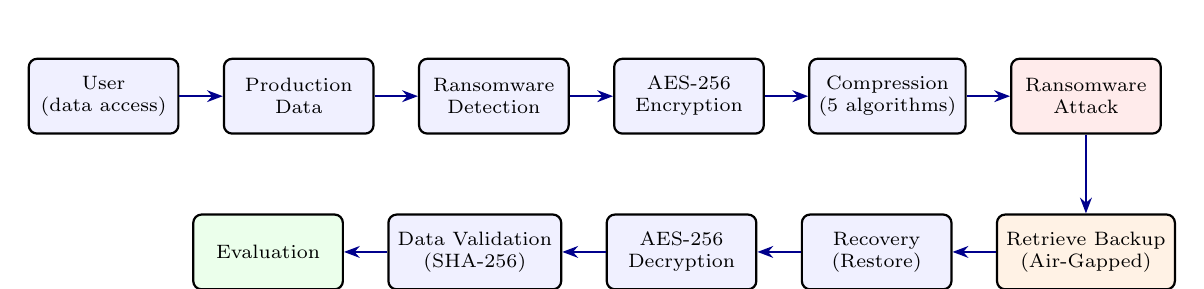
\begin{tikzpicture}[
    font=\scriptsize,
    node distance=0.45cm and 0.55cm,
    stage/.style={draw, rounded corners=3pt, minimum width=1.9cm, minimum height=0.95cm,
                  align=center, fill=blue!6, thick},
    ar/.style={-{Stealth[length=2mm]}, thick, blue!55!black}
]
% Top row (forward flow: backup)
\node[stage] (user)  {User\\(data access)};
\node[stage, right=of user] (prod)  {Production\\Data};
\node[stage, right=of prod] (det)   {Ransomware\\Detection};
\node[stage, right=of det]  (enc)   {AES-256\\Encryption};
\node[stage, right=of enc]  (comp)  {Compression\\(5 algorithms)};
\node[stage, right=of comp, fill=red!8] (atk) {Ransomware\\Attack};
% top row arrows
\foreach \a/\b in {user/prod, prod/det, det/enc, enc/comp, comp/atk}
   \draw[ar] (\a) -- (\b);
% down to bottom row
\node[stage, below=1.0cm of atk, fill=orange!10] (bkp) {Retrieve Backup\\(Air-Gapped)};
\draw[ar] (atk) -- (bkp);
% Bottom row (return flow: recovery) - right to left
\node[stage, left=of bkp]  (rest) {Recovery\\(Restore)};
\node[stage, left=of rest] (dec)  {AES-256\\Decryption};
\node[stage, left=of dec]  (val)  {Data Validation\\(SHA-256)};
\node[stage, left=of val, fill=green!8]  (eval) {Evaluation};
\foreach \a/\b in {bkp/rest, rest/dec, dec/val, val/eval}
   \draw[ar] (\a) -- (\b);
\end{tikzpicture}
\vspace{.7em}
\caption{Proposed system architecture integrating AES-256 encryption, multi-algorithm compression, and air-gapped backup for ransomware protection}
\label{fig:architecture}
\end{figure}

At the storage and detection layer, encrypted and compressed files are stored in an \textit{air-gapped} environment to ensure physical isolation from the production network and enhance resilience against ransomware attacks. In addition, backup data are synchronized to cloud storage (the Google Drive API in the original implementation, or Amazon S3 in the cloud-based replication) for redundancy. Critical metadata, including file size, processing time, and SHA-256 \textit{hash} values, are recorded for performance analysis, integrity verification, and anomaly detection. When ransomware activity is detected, the system automatically initiates a restore process from \textit{air-gapped} storage, followed by decompression and AES-256 decryption to recover files to their original state.

\subsection{Dataset and data acquisition}
The dataset used in this study consists of synthetically generated data designed to resemble real-world enterprise and financial backup structures adapted from the operational environment of PT Equnix. No real financial or confidential production data were used in this study, in order to maintain data privacy and confidentiality compliance \cite{27}.

\begin{table}[H]
\centering
\fontsize{8pt}{10pt}\selectfont
\caption{Characteristics of the dataset used in the experiments}
\label{tab:dataset}
\begin{tabularx}{\textwidth}{@{}c p{1.9cm} p{1.4cm} c p{2.0cm} X@{}}
\hline
\textbf{No} & \textbf{Data Type} & \textbf{File Format} & \textbf{Number of Files} & \textbf{File Size Range} & \textbf{Description} \\
\hline
1 & Structured transaction data & CSV & 9 files & 500 KB -- 1 GB & Used to evaluate compression performance on structured text data with repetitive patterns; file sizes are gradually varied to analyze compression ratio and processing time from small to large scale. \\
2 & System log data & TXT / LOG & 9 files & 500 KB -- 1 GB & Represents application logs and audit trails with repetitive text structures; also used in ransomware attack simulations as logs are common targets. \\
3 & Visual documents & JPG & 14 files & 154 -- 249 KB & Represents binary files with inherent compression, used to evaluate limitations of compression algorithms on already compressed data. \\
4 & Spreadsheet documents & XLSX & 11 files & 500 KB -- 650 MB & Represents operational and financial reports commonly used in financial information systems. \\
\hline
\multicolumn{3}{@{}l}{\textbf{Total}} & \textbf{43 files} & & \\
\hline
\end{tabularx}
\end{table}

The dataset includes various file formats such as CSV, LOG/TXT, JPG, and XLSX with diverse file sizes. This diversity enables a comprehensive evaluation across different data types and storage scales, reflecting practical cloud-based financial systems and supporting ransomware simulation scenarios \cite{35}.

The use of a synthetic \textit{dataset} in this study is a deliberate choice grounded in several considerations. First, currently available public ransomware \textit{datasets}---such as collections of \textit{behavioral} and \textit{API-call} samples for training detection models---are designed for \textit{malware} classification tasks, not for evaluating \textit{backup} and recovery systems that require \textit{victim} document files (CSV, logs, images, and \textit{spreadsheets}) to be backed up and then corrupted in a controlled manner. Consequently, no suitable standard benchmark \textit{dataset} exists for the \textit{backup-recovery} scenario addressed in this study. Second, the use of actual production financial data is not possible for reasons of privacy and confidentiality. Third, a synthetic \textit{dataset} provides full control over file types, sizes, and content patterns, so that compression and recovery performance can be tested systematically and reproducibly. Nevertheless, the authors recognize that a limited-size synthetic \textit{dataset} (43 files) constrains the generalizability of the results; this limitation is discussed in the conclusion as a direction for future work, including the possibility of additional validation using a standard public compression corpus (e.g., the \textit{Silesia Compression Corpus}) that can be reproduced by other researchers.

\subsection{AES-256 encryption and decryption implementation}
To ensure data confidentiality, the system implements the \textit{Advanced Encryption Standard} (AES) with a 256-bit key as a symmetric encryption algorithm. During the backup process, the original file (\textit{plaintext}) is compressed first, and the compressed output is then encrypted using an AES-256 secret key, producing unreadable \textit{ciphertext}. This compressed-and-encrypted file is then stored in \textit{air-gapped} and cloud storage. During the restore process, the file is retrieved from storage, followed by decompression and decryption using the same key to convert the \textit{ciphertext} back into \textit{plaintext}. Data integrity is subsequently verified using SHA-256 \textit{hashing} to ensure that no corruption or unauthorized modification has occurred.

\begin{figure}[H]
\centering
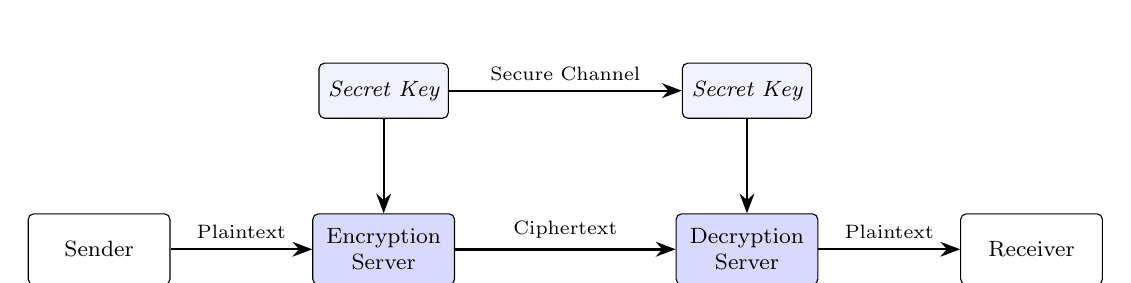
\begin{tikzpicture}[
    node distance=1.4cm and 1.8cm,
    box/.style={draw, rounded corners=2pt, minimum width=1.8cm, minimum height=0.9cm, align=center, font=\footnotesize},
    keyb/.style={draw, rounded corners=2pt, minimum width=1.6cm, minimum height=0.7cm, align=center, font=\footnotesize\itshape, fill=blue!5},
    ar/.style={-{Stealth[length=2.5mm]}, thick},
    font=\footnotesize
]
% bottom row: data flow
\node[box] (sender) {Sender};
\node[box, right=of sender, fill=blue!15] (enc) {Encryption\\Server};
\node[box, right=2.8cm of enc, fill=blue!15] (dec) {Decryption\\Server};
\node[box, right=of dec] (recv) {Receiver};
% top row: keys
\node[keyb, above=1.2cm of enc] (k1) {Secret Key};
\node[keyb, above=1.2cm of dec] (k2) {Secret Key};
% data arrows
\draw[ar] (sender) -- node[above]{\scriptsize Plaintext} (enc);
\draw[ar, line width=1pt] (enc) -- node[above]{\scriptsize Ciphertext} (dec);
\draw[ar] (dec) -- node[above]{\scriptsize Plaintext} (recv);
% key arrows
\draw[ar] (k1) -- node[above, font=\scriptsize]{Secure Channel} (k2);
\draw[ar] (k1) -- (enc);
\draw[ar] (k2) -- (dec);
\end{tikzpicture}
\vspace{.7em}
\caption{AES-256 encryption and decryption process using a symmetric secret key}
\label{fig:aes}
\end{figure}

\subsection{Compression algorithm implementation}
The adaptive compression mechanism implemented in this study uses a rule-based selection strategy (\textit{rule-based decision tree}) rather than \textit{machine learning}. This choice is deliberate: deterministic rules offer low computational \textit{overhead}, a lightweight implementation, and fast, predictable decisions---qualities that are important for cloud backup environments that demand low latency. The algorithm is selected automatically based on file type and size. To be reproducible by other researchers, the complete rules used are summarized explicitly in Table~\ref{tab:rule_selection}. The principle is: small-to-medium text files (CSV, LOG, TXT $\leq 100$ MB) are directed to Snappy or LZ4 for speed; large text files ($> 100$ MB) to Zstandard for a higher compression ratio; already-compressed binary files such as JPG to lightweight algorithms to avoid wasted \textit{overhead}; and XLSX files to LZ4 or Zstandard depending on size. To guarantee that every file is always backed up, the system applies a priority order with a \textit{fallback} mechanism: if a preferred algorithm is unavailable in a given environment, the system automatically switches to the next one, with Gzip as the final safety net since it is always available.

\begin{table}[H]
\centering
\fontsize{8pt}{10pt}\selectfont
\caption{Compression algorithm selection rules by file type and size (priority order with \textit{fallback})}
\label{tab:rule_selection}
\begin{tabular}{l l l}
\hline
\textbf{File type} & \textbf{Size condition} & \textbf{Algorithm priority order} \\
\hline
CSV / LOG / TXT & $\leq 100$ MB & Snappy $\rightarrow$ LZ4 $\rightarrow$ Zstandard \\
CSV / LOG / TXT & $> 100$ MB & Zstandard $\rightarrow$ Gzip \\
JPG & all sizes & Snappy $\rightarrow$ LZ4 $\rightarrow$ Gzip \\
XLSX & $\leq 250$ MB & LZ4 $\rightarrow$ Zstandard \\
XLSX & $> 250$ MB & Zstandard $\rightarrow$ Gzip \\
Others & all sizes & Gzip (\textit{fallback}) \\
\hline
\end{tabular}
\end{table}

The system implements five open-source \textit{lossless} compression algorithms Gzip, Zstandard, Brotli, LZ4, and Snappy to evaluate their performance in a cloud-based backup environment \cite{36}. Gzip is selected for its wide compatibility, while Zstandard and Brotli are used for their high compression ratios. In contrast, LZ4 and Snappy are employed for their high processing speed and low latency characteristics \cite{37}. The implementation is developed in Python, where each dataset file is compressed independently using all five algorithms under identical experimental conditions \cite{38}. Performance evaluation includes compression ratio and processing time measurements to provide a comprehensive analysis of storage efficiency and computational performance \cite{39}, as well as implementation flexibility for hybrid \textit{edge}-cloud backup systems \cite{22}.

\subsection{Backup and recovery procedure}
The backup process begins with SHA-256 \textit{hash} computation to establish a data integrity baseline. Files are then compressed using the selected \textit{lossless} algorithm, followed by encryption of the compressed output using AES-256 to ensure confidentiality (\textit{compress-then-encrypt}). The resulting files are temporarily stored in an \textit{air-gapped} directory before being transferred to cloud storage. In addition to the \textit{air-gapped} mechanism, a \textit{mirroring} strategy is implemented to enhance data availability and recovery readiness. Under normal conditions, when no anomalies or ransomware indicators are detected based on \textit{hash} and metadata verification, the system terminates after completing the backup process without initiating recovery. This approach minimizes unnecessary recovery operations and reduces system \textit{overhead}.

The recovery process is triggered only when anomalies are detected, such as \textit{hash} mismatches, metadata inconsistencies, or indications of unauthorized encryption. In such cases, data are retrieved from \textit{air-gapped} storage, decrypted first, and then decompressed to restore the original files (the reverse of the backup order). The recovered files are then validated by comparing their \textit{hash} values against the reference baseline.

\begin{figure}[H]
\centering
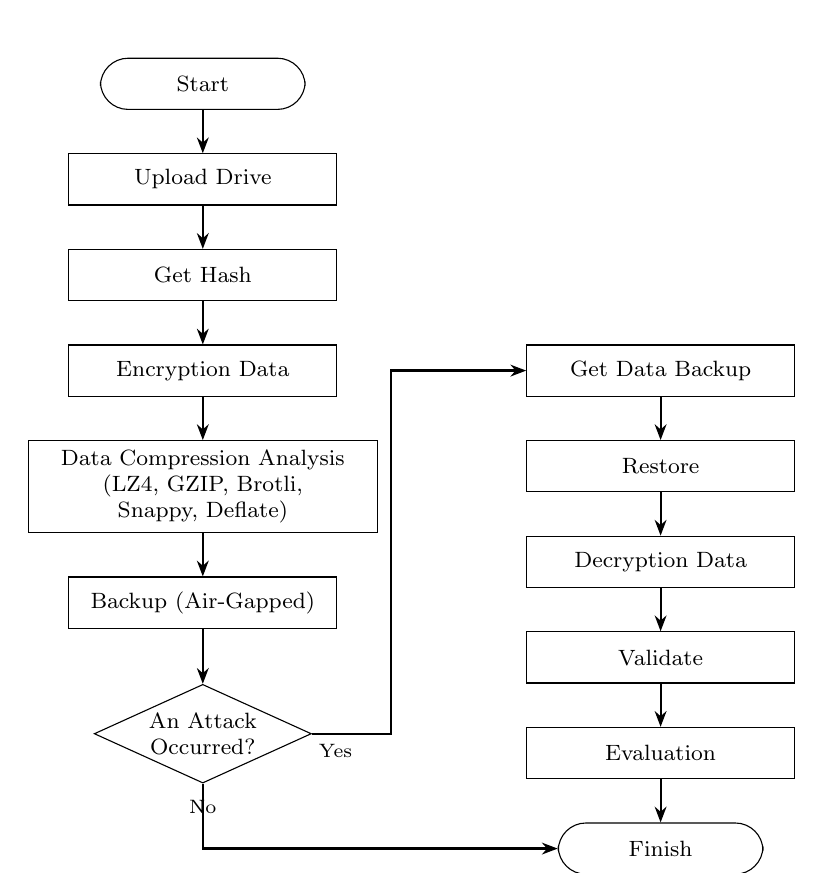
\begin{tikzpicture}[
    node distance=0.55cm,
    every node/.style={font=\footnotesize},
    term/.style={draw, rounded corners=10pt, minimum width=2.6cm, minimum height=0.65cm, align=center},
    proc/.style={draw, minimum width=3.4cm, minimum height=0.65cm, align=center},
    dec/.style={draw, diamond, aspect=2.2, inner sep=1pt, align=center},
    ar/.style={-{Stealth[length=2mm]}, thick}
]
% ----- Left column: backup flow -----
\node[term] (start) {Start};
\node[proc, below=of start] (upload) {Upload Drive};
\node[proc, below=of upload] (hash) {Get Hash};
\node[proc, below=of hash] (enc) {Encryption Data};
\node[proc, below=of enc, text width=4.2cm] (comp) {Data Compression Analysis\\(LZ4, GZIP, Brotli, Snappy, Deflate)};
\node[proc, below=of comp] (backup) {Backup (Air-Gapped)};
\node[dec, below=0.7cm of backup] (att) {An Attack\\Occurred?};
% ----- Right column: recovery flow (top-aligned with start) -----
\node[proc, right=2.4cm of enc] (getbk) {Get Data Backup};
\node[proc, below=of getbk] (restore) {Restore};
\node[proc, below=of restore] (decr) {Decryption Data};
\node[proc, below=of decr] (valid) {Validate};
\node[proc, below=of valid] (eval) {Evaluation};
\node[term, below=of eval] (finish) {Finish};
% left column arrows
\draw[ar] (start) -- (upload);
\draw[ar] (upload) -- (hash);
\draw[ar] (hash) -- (enc);
\draw[ar] (enc) -- (comp);
\draw[ar] (comp) -- (backup);
\draw[ar] (backup) -- (att);
% decision Yes -> enter recovery column at the top (Get Data Backup)
\draw[ar] (att.east) -- node[below, font=\scriptsize, pos=0.3]{Yes} ++(1.0cm,0) |- (getbk.west);
% right column arrows
\draw[ar] (getbk) -- (restore);
\draw[ar] (restore) -- (decr);
\draw[ar] (decr) -- (valid);
\draw[ar] (valid) -- (eval);
\draw[ar] (eval) -- (finish);
% decision No -> skip recovery, go straight to Finish (enter from the left edge)
\draw[ar] (att.south) |- node[below, font=\scriptsize, pos=0.05]{No} (finish.west);
\end{tikzpicture}
\vspace{.7em}
\caption{Backup and recovery system flowchart}
\label{fig:backup_flow}
\end{figure}

\subsection{Ransomware attack simulation}
To evaluate the resilience of the proposed backup system, a ransomware attack simulation was conducted without executing actual \textit{malware}. This simulation was based on real-world vulnerability patterns, including CVE-2017-0144, which represents an \textit{encrypt-and-hold} attack model; CVE-2021-36934, which simulates file overwriting and corruption behavior; and CVE-2018-8453, which targets file metadata and \textit{header} structure. In each scenario, file modifications were carried out in a controlled manner to mimic ransomware-induced damage. The objective of this simulation is to assess the system's ability to detect anomalies and to recover affected files from \textit{air-gapped} backups.

\subsection{Ransomware detection and encryption differentiation mechanism}
In modern cloud systems, files may undergo legitimate compression and encryption processes, which must be differentiated from ransomware-induced encryption. The detection mechanism in this study combines SHA-256 \textit{hash} verification, metadata analysis, and \textit{air-gapped} backup validation. Each file's \textit{hash} is computed as an integrity baseline and re-verified during inspection to detect unauthorized changes. In addition, metadata consistency such as file size, modification time, file type, and extension is analyzed alongside file structure characteristics to identify abnormal changes inconsistent with legitimate AES-256 encryption or compression processes.

If discrepancies are detected between primary storage and the \textit{air-gapped} backup copies, the system classifies the condition as a potential compromise. Based on the results of \textit{hash}, metadata, and backup validation, files are categorized as normal condition, legitimate modification, or ransomware indication, enabling early detection and secure data recovery.

\subsection{Performance evaluation metrics}
The performance of the cloud-based backup system with multi-algorithm compression is evaluated through quantitative experimental analysis. Several metrics are used to assess storage efficiency, processing performance, data integrity, and system resilience. The \textit{Compression Ratio} (CR) is defined as:

\begin{equation}
CR = \frac{S_{after}}{S_{before}}
\end{equation}

where $S_{before}$ represents the file size before compression and $S_{after}$ represents the file size after compression. Compression Factor (CF) indicates how many times the original data size is reduced after compression and is the inverse of the compression ratio. A higher CF value indicates better compression efficiency:

\begin{equation}
CF = \frac{S_{before}}{S_{after}}
\end{equation}

Storage Saving Percentage (SS) is used to measure the percentage of storage space saved after compression, which is particularly important in long-term cloud storage scenarios:

\begin{equation}
SS = \frac{S_{before} - S_{after}}{S_{before}} \times 100\%
\end{equation}

To comprehensively evaluate compression algorithm efficiency, this study introduces a combined efficiency score ($E$) that integrates storage efficiency and compression time efficiency. This score is calculated using a Multi-Criteria Decision Making (MCDM) approach with the Weighted Sum Model (WSM), formulated as:

\begin{equation}
E = \alpha (1 - R) + \beta \left( \frac{1}{T} \right)
\end{equation}

where $R$ denotes the compression ratio, with $(1-R)$ representing storage efficiency, and $T$ represents compression time in seconds, with $1/T$ indicating processing time efficiency. The parameters $\alpha$ and $\beta$ are weighting factors that control the contribution of each component, set to $\alpha = 0.5$ and $\beta = 0.5$ to ensure a balanced evaluation between storage efficiency and processing speed. To enable relative comparison among algorithms, the combined efficiency score is normalized as follows:

\begin{equation}
E(\%) = \frac{E}{E_{max}} \times 100
\end{equation}

The interpretation of the combined efficiency score is based on the performance classification shown in Table~\ref{tab:efficiency_criteria}.

\begin{table}[H]
\centering
\fontsize{8pt}{10pt}\selectfont
\caption{Criteria for interpreting system efficiency score}
\label{tab:efficiency_criteria}
\begin{tabularx}{\textwidth}{@{}c c X@{}}
\hline
\textbf{Score (\%)} & \textbf{Status} & \textbf{Description} \\
\hline
$\geq 90$ & Excellent & Very high performance in both storage efficiency and processing speed \\
80--89 & Good & Strong performance suitable for high-performance systems \\
70--79 & Fair & One aspect is dominant while the other is relatively weaker \\
$< 70$ & Poor & Overall efficiency is low \\
\hline
\end{tabularx}
\end{table}

In addition to compression efficiency metrics, this study also evaluates system recovery performance as part of overall system resilience. The Recovery Time Objective (RTO) represents the total time required for the system to restore normal operation after a ransomware attack is detected:

\begin{equation}
RTO = T_{recovery} - T_{incident}
\end{equation}

where $T_{incident}$ is the time when the ransomware attack is identified, and $T_{recovery}$ is the time when the system has fully recovered. A lower RTO indicates faster recovery performance and higher system resilience. To evaluate the reliability of ransomware detection, this study also measures False Positive Rate (FPR) and False Negative Rate (FNR). These metrics are used to assess the capability of the system in distinguishing legitimate backup encryption activities from unauthorized ransomware-induced modifications. False Positive Rate (FPR) is defined as:

\begin{equation}
FPR = \frac{FP}{FP + TN} \times 100\%
\end{equation}

False Negative Rate (FNR) is defined as:

\begin{equation}
FNR = \frac{FN}{FN + TP} \times 100\%
\end{equation}

where FP represents False Positive cases, where normal files are incorrectly identified as ransomware; TN represents True Negative cases, where normal files are correctly identified as safe; FN represents False Negative cases, where ransomware-infected files are not detected; and TP represents True Positive cases, where ransomware-infected files are successfully detected. Lower FPR and FNR values indicate higher reliability of the detection mechanism and better system resilience against ransomware attacks.

\section{Results and Discussion}
\label{sec:results}
Experimental results show that the proposed cloud backup system provides reliable data protection, compression, and recovery performance. All files maintained identical SHA-256 hash values, indicating zero data alteration. Zstandard achieved the highest compression efficiency, while Snappy and LZ4 provided the fastest processing time. During ransomware simulation, the air-gapped mechanism enabled 100\% successful recovery with zero errors, demonstrating strong system resilience.

\subsection{Experimental environment}
To test both reliability and cross-platform consistency, the system was evaluated in two environments: (1) a local \textbf{Windows}-based development environment, and (2) a \textbf{cloud}-based replication environment on Amazon Web Services (AWS) EC2 covering Windows Server and Linux instances. Replication in the \textit{cloud} environment is highly relevant because the proposed system is indeed intended for cloud-based backup deployment. The configurations of both environments are summarized in Table~\ref{tab:experimental_setup}.

\begin{table}[H]
\centering
\fontsize{8pt}{10pt}\selectfont
\caption{Experimental setup across two test environments}
\label{tab:experimental_setup}
\begin{tabularx}{\textwidth}{@{}l X X@{}}
\hline
\textbf{Component} & \textbf{Local Environment (Windows)} & \textbf{Cloud Environment (AWS EC2)} \\
\hline
Operating System & Windows 11 (64-bit) & Windows Server 2022 \& Ubuntu 22.04 \\
CPU & Intel Core i7-11800H (8-core) & t3.xlarge (4 vCPU) / t3.large (2 vCPU) \\
RAM & 16 GB & 16 GB (Windows) / 8 GB (Linux) \\
Programming Language & Python 3.10 & Python 3.11 (Windows) / 3.10 (Linux) \\
Compression Libraries & \multicolumn{2}{l}{Gzip, Zstandard, Brotli, LZ4, Snappy} \\
Cryptography Libraries & \multicolumn{2}{l}{PyCryptodome (AES-256), hashlib (SHA-256)} \\
\textit{Air-gapped} Media & External SSD / VHDX (separate disk) & Separate EBS volume (drive D: / \texttt{/mnt/airgap}) \\
Cloud Storage & Google Drive API & Amazon S3 \\
\hline
\end{tabularx}
\end{table}

The local Windows environment is the \textbf{initial development environment} where the system was first designed and implemented; its configuration represents a mid-to-high performance consumer computer commonly used in enterprise backup systems. The AWS EC2 environment, meanwhile, is the \textbf{primary measurement and validation environment} that represents a real \textit{cloud} deployment---consistent with the system's goal as a cloud-based backup. To maintain consistency and honest reporting, all quantitative figures reported in this section (compression ratio, \textit{throughput}, recovery time/RTO, and repeated-trial statistics) were obtained from controlled measurements on the AWS EC2 environment. In the \textit{cloud} environment, the \textit{air-gapped} media is realized as a separate EBS volume that is only mounted during the backup/recovery process, mimicking the logical isolation of the media in the local environment. Testing in two environments allows verification that the system's results are \textbf{consistent across platforms} (Windows and Linux), while also addressing the generalizability limitation common to studies tested on a single platform.

\subsection{System simulation results under normal conditions (no attack)}
Evaluation under normal conditions focuses on the system's main workflow, including cloud storage connection initialization, compression using multiple \textit{lossless} algorithms, secure backup storage, and data integrity validation.

\subsubsection{Cloud storage connection initialization}
As shown in Figure~\ref{fig:drive_conn}, the system successfully establishes a secure connection to cloud storage using a token/role-based authentication mechanism (OAuth~2.0 in the Google Drive implementation, or an IAM \textit{role} in the Amazon S3-based replication). Each backup session generates a unique session ID, ensuring that all operations are performed within an authenticated environment. This result indicates that the system provides secure access control, preventing unauthorized interactions with cloud storage during the backup process.

\begin{figure}[H]
\centering
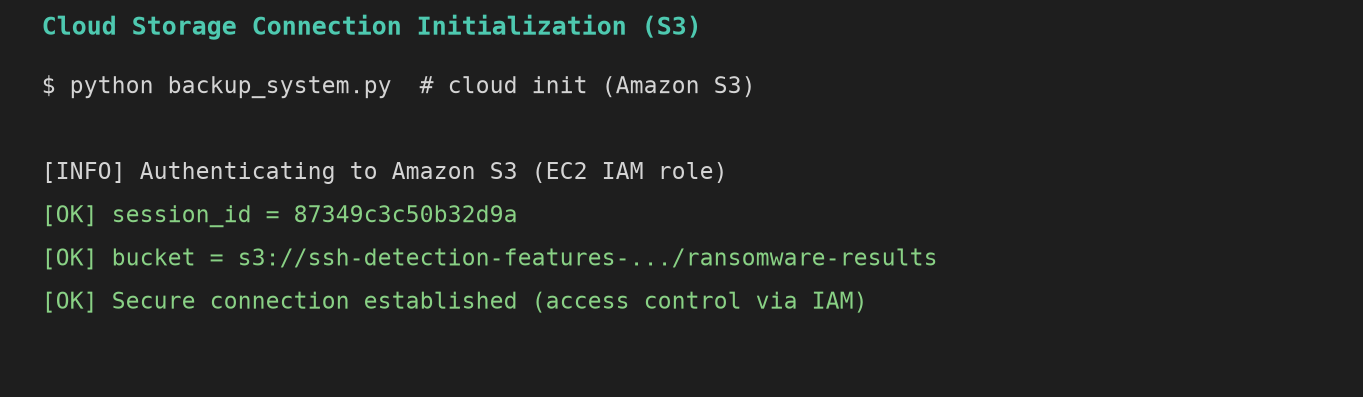
\includegraphics[width=\textwidth]{figures/figure4_cloud_conn_en.png}
\vspace{.7em}
\caption{Drive connection results (session ID)}
\label{fig:drive_conn}
\end{figure}

This successful authentication demonstrates that the backup mechanism can securely establish communication with cloud storage while preventing unauthorized access. The use of unique session IDs also improves traceability and auditing capability, which is important in backup systems handling sensitive data.

\subsubsection{File upload and deduplication process}
As shown in Figure~\ref{fig:upload}, the system performs file upload followed by initial validation using SHA-256 \textit{hashing} and metadata verification before proceeding to compression and encryption. This process ensures that only valid and verified files are processed, reducing redundancy and improving storage efficiency. Early validation also helps detect inconsistencies before backup is performed, thereby strengthening overall data integrity.

\begin{figure}[H]
\centering
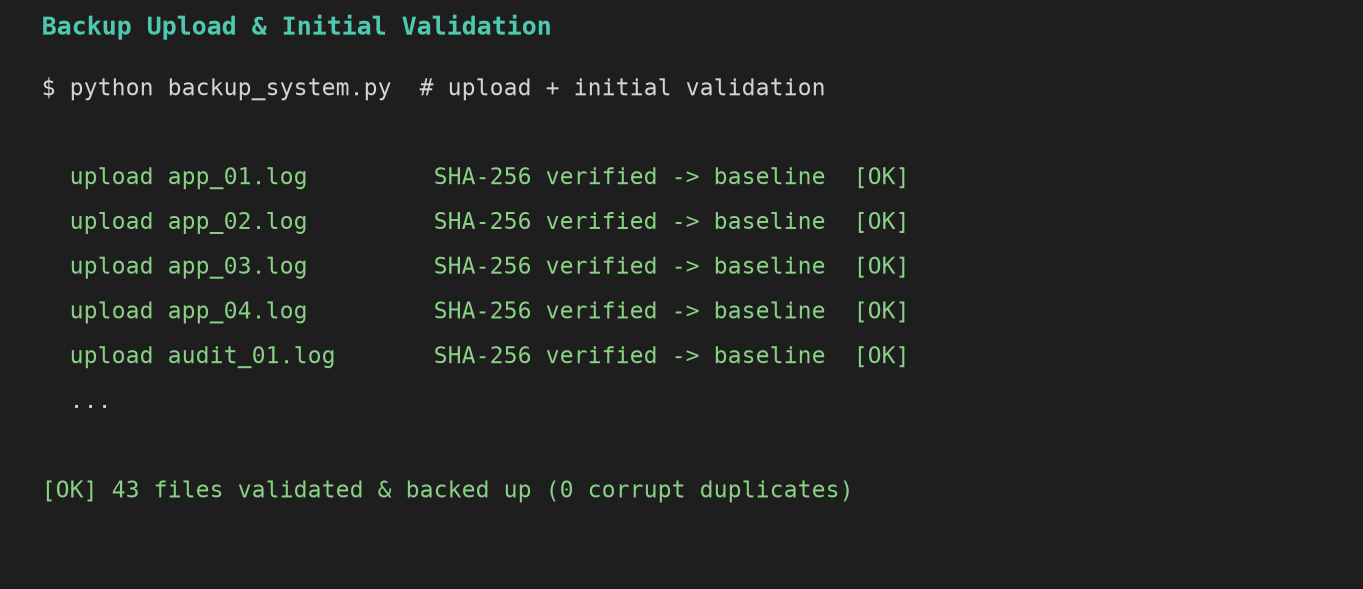
\includegraphics[width=\textwidth]{figures/figure5_upload_en.png}
\vspace{.7em}
\caption{Backup upload and initial validation results}
\label{fig:upload}
\end{figure}

The validation process before compression reduces the possibility of storing duplicated or corrupted files. It contributes to storage efficiency and minimizes unnecessary backup operations, particularly for large-scale backup environments.

\subsubsection{Hash and metadata validation}
As shown in Figure~\ref{fig:sha_json}, the system performs integrity validation using the SHA-256 \textit{hashing} algorithm to ensure that file content remains unchanged during the backup process. Each uploaded file is processed to generate a unique \textit{hash} value that serves as a digital fingerprint for integrity verification.

\begin{figure}[H]
\centering
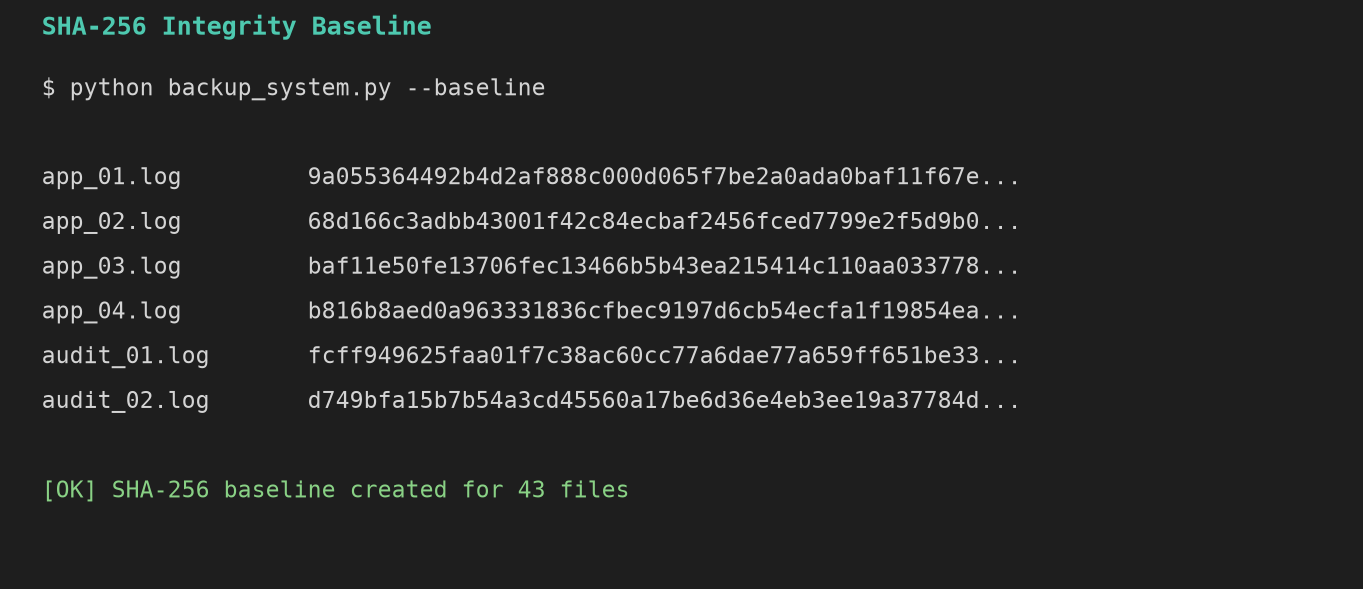
\includegraphics[width=\textwidth]{figures/figure6_sha256_en.png}
\vspace{.7em}
\caption{SHA-256 results for the JSON file}
\label{fig:sha_json}
\end{figure}

In addition to \textit{hash} verification, the system validates metadata such as file size, last modified timestamp, MIME type, file extension, and basic file structure. All this information, including the \textit{hash} value, is stored in JSON format as a baseline reference before backup, as shown in Figure~\ref{fig:metadata}.

\begin{figure}[H]
\centering
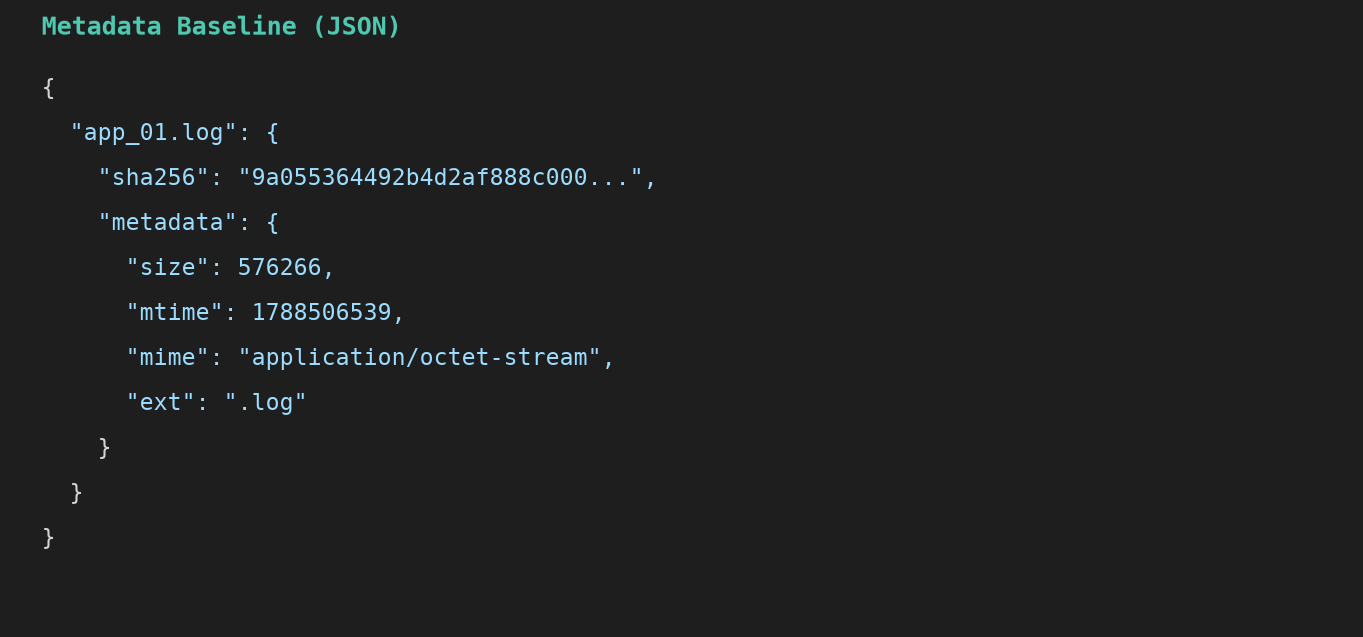
\includegraphics[width=0.8\textwidth]{figures/figure7_metadata.png}
\vspace{.7em}
\caption{Metadata results in JSON format}
\label{fig:metadata}
\end{figure}

The baseline validation mechanism is designed to support integrity verification throughout the compression, encryption, storage, and recovery stages. Matching \textit{hash} values and metadata indicate that no unauthorized modifications occur in either file content or file structure. The validation process used in this study is summarized in Algorithm 1.

\begin{table}[H]
\centering
\fontsize{8pt}{10pt}\selectfont
\begin{tabularx}{\textwidth}{@{}X@{}}
\hline
\textbf{Algorithm 1. Hash and metadata validation process} \\
\hline
FOR each file IN dataset: \\
\quad hash = SHA256(file) \\
\quad metadata = extract\_metadata(file) \\
\quad IF hash or metadata differ from baseline: mark\_as\_anomaly(file) \\
\quad ELSE: mark\_as\_safe(file) \\
\hline
\end{tabularx}
\end{table}

The algorithm combines hash-based verification with metadata comparison to improve anomaly detection capability. This approach allows the system to identify not only content-level modifications but also structural changes commonly caused by ransomware attacks, such as altered timestamps, suspicious extensions, or corrupted file headers.

\begin{figure}[H]
\centering
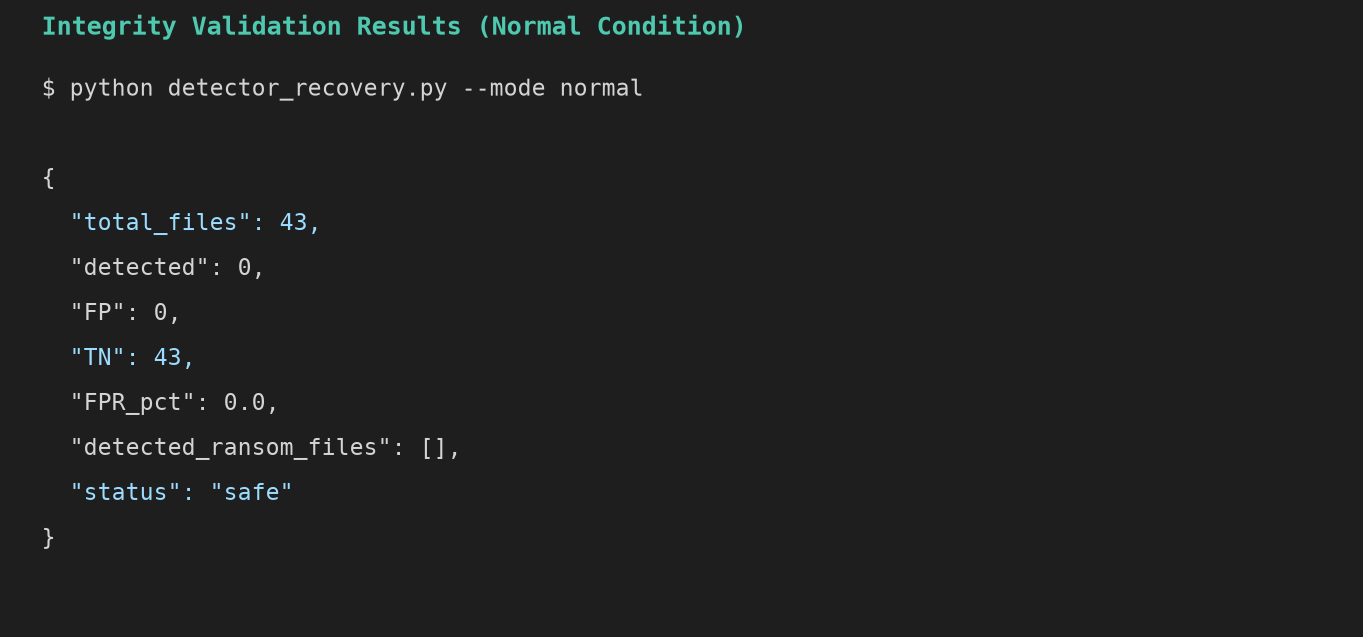
\includegraphics[width=0.8\textwidth]{figures/figure8_validation_en.png}
\vspace{.7em}
\caption{Validation results of SHA-256 hash and file metadata}
\label{fig:validation}
\end{figure}

Figure~\ref{fig:validation} presents the validation results generated by the system. The output shows that all files were successfully verified and no ransomware indicators were detected, as indicated by the value \texttt{detected\_ransom\_files: []}. This result confirms that all files were in a safe condition before entering the compression and encryption stages. Furthermore, the absence of anomalies demonstrates that the integrity validation mechanism can effectively distinguish normal files from suspicious modifications.

\subsubsection{AES-256 encryption implementation}
To enhance data security, the system applies the \textit{Advanced Encryption Standard} (AES-256) before storing files as backups. Verified files are processed using a previously stored encryption key, producing encrypted files with the \texttt{.enc} extension. AES-256 provides a high level of security with a 256-bit key length, protecting data confidentiality from unauthorized access.

\begin{figure}[H]
\centering
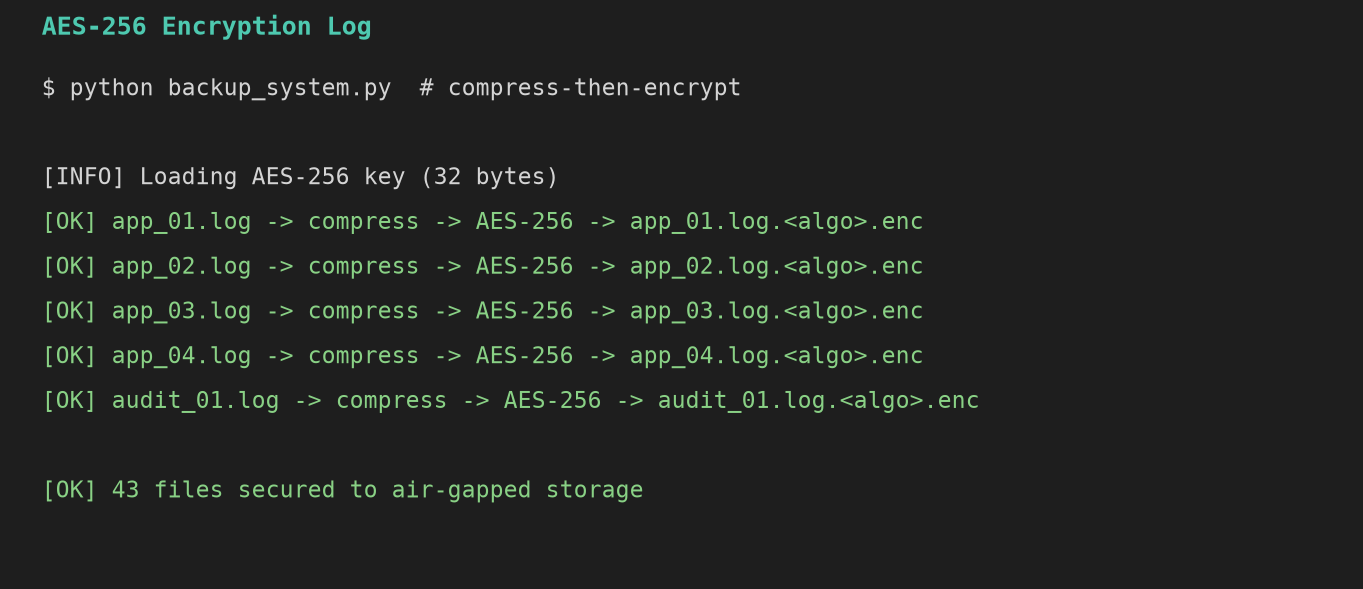
\includegraphics[width=\textwidth]{figures/figure9_aeslog_en.png}
\vspace{.7em}
\caption{Log of the file encryption implementation using the AES-256 algorithm}
\label{fig:aes_log}
\end{figure}

Figure~\ref{fig:aes_log} shows the AES-256 encryption implementation log, including encryption key loading, file encryption execution, and successful encrypted file creation. This confirms that encryption operates properly and is an integral part of the cloud backup system's security. The encryption workflow implemented in the system is summarized in Algorithm 2.

\begin{table}[H]
\centering
\fontsize{8pt}{10pt}\selectfont
\begin{tabularx}{\textwidth}{@{}X@{}}
\hline
\textbf{Algorithm 2. AES-256 encryption process} \\
\hline
LOAD encryption\_key \\
FOR each validated\_file IN dataset: \\
\quad encrypted\_file = AES256\_Encrypt(validated\_file, encryption\_key) \\
\quad save(encrypted\_file, ".enc") \\
\quad log\_encryption\_status(encrypted\_file) \\
\hline
\end{tabularx}
\end{table}

Encryption process is performed only after hash and metadata validation are successfully completed. This approach ensures that the system can distinguish legitimate backup encryption from abnormal file modifications caused by ransomware. Unlike ransomware behavior, the encryption mechanism in this study operates within a controlled environment using authorized encryption keys and verified files.

\subsection{Compression performance results by algorithm}
Performance evaluation was conducted on the four file types (CSV, Log/TXT, JPG, and XLSX) using the five \textit{lossless} algorithms. Table~\ref{tab:compression_results} presents the average storage saving percentage (\textit{storage saving}, SS) measured at the \textit{plaintext} compression stage (before encryption) for each combination of file type and algorithm.

\begin{table}[H]
\centering
\fontsize{8pt}{10pt}\selectfont
\caption{Average storage saving (\%) by file type and algorithm (experimental results, 43 files)}
\label{tab:compression_results}
\begin{tabular}{l c c c c c}
\hline
\textbf{File Type} & \textbf{Gzip} & \textbf{Zstandard} & \textbf{Brotli} & \textbf{LZ4} & \textbf{Snappy} \\
\hline
Log/TXT & 88.5 & 87.6 & \textbf{89.5} & 77.4 & 80.2 \\
CSV     & 79.9 & 78.7 & \textbf{81.1} & 66.6 & 66.4 \\
XLSX    & 1.1  & 0.0  & 0.0  & 0.0  & 0.0  \\
JPG     & 0.1  & 0.0  & 0.0  & 0.0  & 0.0  \\
\hline
\end{tabular}
\end{table}

Table~\ref{tab:compression_results} confirms the relationship between data entropy and compression ratio. Low-entropy text files with repetitive patterns yield the highest savings: Log/TXT reaches up to \textbf{89.5\%} and CSV up to \textbf{81.1\%} (Brotli), with Gzip and Zstandard following very closely (above 78\%). The fast algorithms LZ4 and Snappy yield slightly lower savings (66--80\%) but with far shorter processing times, making them a balanced choice for real-time scenarios. Conversely, JPG files (\textit{lossy}, already compressed) and XLSX files (already-\textit{deflated} ZIP containers) approach \textbf{0\%} savings across all algorithms, confirming the limitations of \textit{lossless} compression on high-entropy data. These findings validate the rationale of the rule-based adaptive selection mechanism: fast algorithms (Snappy/LZ4) are chosen for small-to-medium files for low latency, while high-ratio algorithms (Zstandard/Brotli) are prioritized for large text files for long-term storage efficiency.

\begin{figure}[H]
\centering
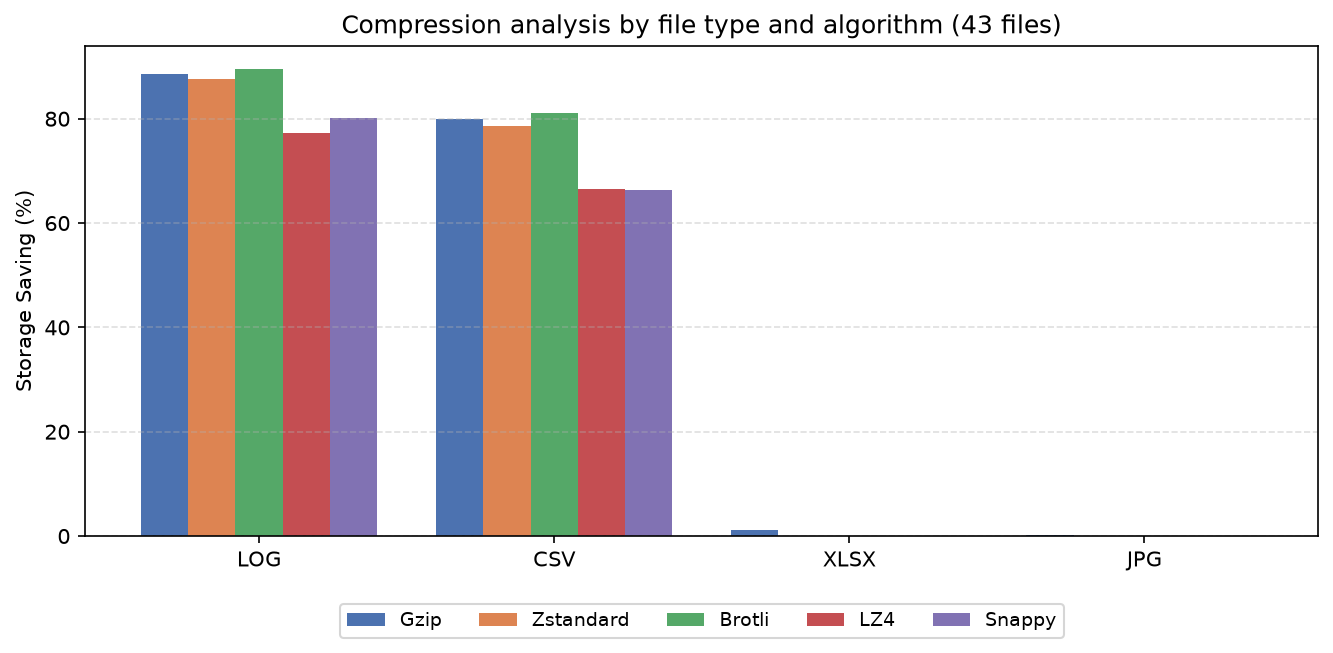
\includegraphics[width=\textwidth]{figures/figure10_compression_en.png}
\vspace{.7em}
\caption{Overall analysis results of the algorithms}
\label{fig:overall_analysis}
\end{figure}

\subsection{Statistical analysis of compression performance}
To strengthen the validity of the results, compression performance measurements were repeated five times (\textit{repeated trials}) on the entire \textit{dataset} (43 files, $\approx 531$ MB) in the AWS EC2 environment (Ubuntu 22.04). Table~\ref{tab:comp_stats} reports the mean and standard deviation (\textit{std}) of compression time, \textit{throughput} (MB/s), and CPU and RAM utilization measured using the \texttt{psutil} library.

\begin{table}[H]
\centering
\fontsize{8pt}{10pt}\selectfont
\caption{Statistical analysis of compression performance (5 \textit{trials}, dataset of 43 files $\approx$531 MB)}
\label{tab:comp_stats}
\begin{tabular}{l c c c c c}
\hline
\textbf{Algorithm} & \textbf{Mean time (s)} & \textbf{Std (s)} & \textbf{Throughput (MB/s)} & \textbf{CPU (\%)} & \textbf{RAM (MB)} \\
\hline
Gzip      & 17.427 & 0.062 & 30.5  & 100.0 & 6.3 \\
Brotli    & 10.468 & 0.237 & 50.7  & 100.0 & 5.1 \\
Zstandard & 1.721  & 0.016 & 308.7 & 99.9  & 3.4 \\
LZ4       & 0.896  & 0.011 & 592.7 & 100.0 & $<$1 \\
Snappy    & 0.831  & 0.003 & 639.0 & 99.3  & 0.9 \\
\hline
\end{tabular}
\end{table}

The very small standard deviation across all algorithms (e.g., Snappy $0.003$ s, Zstandard $0.016$ s) shows that compression performance is \textbf{stable and consistent} across repetitions. There is a wide \textit{throughput} range: Snappy and LZ4 reach $>590$ MB/s---roughly $20\times$ faster than Gzip ($30.5$ MB/s)---while Zstandard offers an attractive balance ($308.7$ MB/s) with a high compression ratio (Table~\ref{tab:compression_results}). CPU utilization near $100\%$ for all algorithms confirms that the compression process is \textit{CPU-bound}, while the memory (RAM) footprint remains small ($<7$ MB), making the system lightweight and suitable for resource-constrained backup environments. These quantitative results provide an objective basis for the adaptive selection mechanism: a combination of high \textit{throughput} (Snappy/LZ4) for small-to-medium files and a balanced ratio-throughput (Zstandard) for large text files.

\subsection{Quantitative comparison of the adaptive strategy against baselines}
To objectively evaluate the benefit of the proposed adaptive selection mechanism, this strategy was compared against three \textit{baseline} strategies on the entire \textit{dataset} (43 files, $\approx 531$ MB): (i) no compression, (ii) single static Gzip compression (a common practice in legacy backup systems), and (iii) single static Zstandard compression. Table~\ref{tab:baseline_comparison} summarizes the results.

\begin{table}[H]
\centering
\fontsize{8pt}{10pt}\selectfont
\caption{Comparison of the adaptive compression strategy against baselines (43 files, $\approx$531 MB)}
\label{tab:baseline_comparison}
\begin{tabular}{l c c c c}
\hline
\textbf{Strategy} & \textbf{Final Size (MB)} & \textbf{Saving (\%)} & \textbf{Time (s)} & \textbf{Throughput (MB/s)} \\
\hline
No compression        & 531.2 & 0.00  & --    & -- \\
Static-Gzip           & 265.1 & 50.09 & 18.84 & 28.2 \\
Static-Zstandard      & 271.1 & 48.96 & 1.94  & 273.8 \\
\textbf{Adaptive (proposed)} & 301.3 & 43.28 & \textbf{0.87} & \textbf{611.8} \\
\hline
\end{tabular}
\end{table}

These results reveal an important \textit{trade-off}. The static Gzip strategy achieves the highest storage saving ($50.1\%$), but at the cost of very high processing time ($18.84$ s; \textit{throughput} of only $28.2$ MB/s). Conversely, the \textbf{proposed adaptive strategy} deliberately prioritizes speed: by selecting fast algorithms (Snappy/LZ4) for most files, it completes the entire process in just $0.87$ s---\textbf{about $21\times$ faster than static Gzip} and $2.2\times$ faster than static Zstandard---while still delivering reasonable storage saving ($43.3\%$). The relatively small difference in saving ($6.8$ percentage points compared with Gzip) is traded for a dramatic \textit{throughput} improvement ($611.8$ vs $28.2$ MB/s). For backup systems that demand a low \textit{Recovery Time Objective} (RTO) and minimal computational \textit{overhead}---especially in resource-constrained environments---this emphasis on speed is more advantageous than maximizing the compression ratio in absolute terms. Thus, the main advantage of the adaptive mechanism is not the absolute saving, but the \textbf{optimal balance between storage efficiency and processing speed} that can be tailored to workload characteristics.

\subsection{Entropy analysis: linking theory to empirical evidence}
To verify the theoretical foundation (Section~1) empirically, the Shannon entropy $H(X)$ (in bits/\textit{byte}, range 0--8) was measured for each file type and related to the achieved storage saving. Table~\ref{tab:entropy_type} presents the results.

\begin{table}[H]
\centering
\fontsize{8pt}{10pt}\selectfont
\caption{Shannon entropy per file type and its relation to storage saving}
\label{tab:entropy_type}
\begin{tabular}{l c c}
\hline
\textbf{File Type} & \textbf{Entropy (bits/byte)} & \textbf{Saving (\%)} \\
\hline
CSV  & 4.573 & 66.4 \\
LOG  & 5.232 & 80.0 \\
XLSX & 7.962 & $\approx$0 \\
JPG  & 7.940 & $\approx$0 \\
\hline
\end{tabular}
\end{table}

These results directly confirm the predictions of information theory: text files (CSV, LOG) have low entropy ($4.6$--$5.2$ bits/\textit{byte}) due to high pattern redundancy and can therefore be compressed by $66$--$80\%$. Conversely, JPG and XLSX files have entropy close to the maximum limit ($\approx 7.95$ bits/\textit{byte}), indicating high randomness because they are already compressed, so their compression ratio is near zero. This strong inverse correlation between entropy and storage saving provides quantitative justification for the file-type-based adaptive selection mechanism.

Furthermore, entropy also serves as an attack indicator. Table~\ref{tab:entropy_attack} compares file entropy before and after a simulated \textit{encrypt-and-hold} attack.

\begin{table}[H]
\centering
\fontsize{8pt}{10pt}\selectfont
\caption{Shannon entropy change before and after ransomware encryption attack}
\label{tab:entropy_attack}
\begin{tabular}{l c c c}
\hline
\textbf{File Type} & \textbf{Before} & \textbf{After} & \textbf{$\Delta H$} \\
\hline
CSV  & 4.547 & 8.000 & $+3.453$ \\
LOG  & 5.223 & 8.000 & $+2.777$ \\
JPG  & 7.940 & 8.000 & $+0.060$ \\
XLSX & 7.963 & 8.000 & $+0.036$ \\
\hline
\end{tabular}
\end{table}

Low-entropy text files experience a sharp entropy spike toward the maximum value ($8.0$ bits/\textit{byte}) after encryption ($\Delta H$ up to $+3.45$ for CSV), a characteristic sign of unauthorized encryption. However, files that already have high entropy (JPG, XLSX) change only slightly, underscoring a fundamental limitation of entropy-based detection: techniques such as \textit{Format-Preserving Encryption} that do not raise entropy can fool it. This finding reinforces the rationale for this study's choice to rely on \textit{hash}- and metadata-based integrity verification---which detects \textit{any} file change regardless of its entropy---instead of depending on entropy alone.

\subsection{Recovery time scalability test}
To evaluate the feasibility of the system at larger scales (addressing enterprise-environment needs), the \textit{backup} and recovery cycle was measured at several total \textit{dataset} sizes from 50 MB to 1 GB. Table~\ref{tab:scalability} presents the results.

\begin{table}[H]
\centering
\fontsize{8pt}{10pt}\selectfont
\caption{Scalability of backup and recovery time (RTO) with respect to dataset size}
\label{tab:scalability}
\begin{tabular}{c c c c}
\hline
\textbf{Dataset Size (MB)} & \textbf{Backup Time (s)} & \textbf{Recovery RTO (s)} & \textbf{Successful Recovery} \\
\hline
51.2   & 0.187 & 0.344 & 8/8 \\
101.1  & 0.339 & 0.699 & 8/8 \\
250.9  & 0.872 & 1.797 & 8/8 \\
500.5  & 1.843 & 4.020 & 8/8 \\
1001.0 & 5.927 & 7.731 & 8/8 \\
\hline
\end{tabular}
\end{table}

The recovery time (RTO) increases \textbf{approximately linearly} with dataset size, at an average rate of $\approx 0.0073$ seconds/MB (standard deviation of only $0.0005$ seconds/MB), confirming the deterministic nature of the recovery workflow (SHA-256 verification, AES-256 decryption, and decompression). Even for a 1 GB \textit{dataset}, full recovery completes in $\approx 7.7$ seconds with integrity perfectly preserved (all files recovered and passing \textit{hash} verification). This linearity enables reliable RTO projection for enterprise-scale workloads: the system stays within an acceptable recovery window as data volume grows.

\subsection{Implementation and structure of air-gapped backup storage}
As an additional layer of protection, the system implements an air-gapped backup mechanism using a separate storage medium in the form of an external SSD. This medium is not permanently accessed by the system but is only mounted during backup or restore processes. This approach aims to minimize the risk of unauthorized access and malware propagation through network channels. The air-gapped implementation used in this study is online (logical air-gapped backup), where the storage medium remains within the system environment through access control settings, active sessions, and limited mounting mechanisms. With this approach, the medium can only be accessed under specific conditions defined by the system, without an active network connection during the backup storage process.

Although the proposed logical air-gapped mechanism significantly reduces ransomware exposure, it does not provide the same level of isolation as a fully offline physical air-gapped infrastructure. Because the backup media is mounted temporarily during backup and recovery sessions, advanced malware capable of memory persistence or delayed execution may still attempt to access the mounted storage once it becomes available. However, this risk is mitigated through temporary mounting duration, automatic disconnection after backup completion, SHA-256 integrity verification, metadata validation, isolated backup repositories, and restricted access sessions. Therefore, the proposed architecture provides a practical and cost-effective ransomware resilience solution suitable for small and medium-sized organizations that may not have sufficient resources to deploy fully physical offline air-gapped infrastructures.

\begin{figure}[H]
\centering
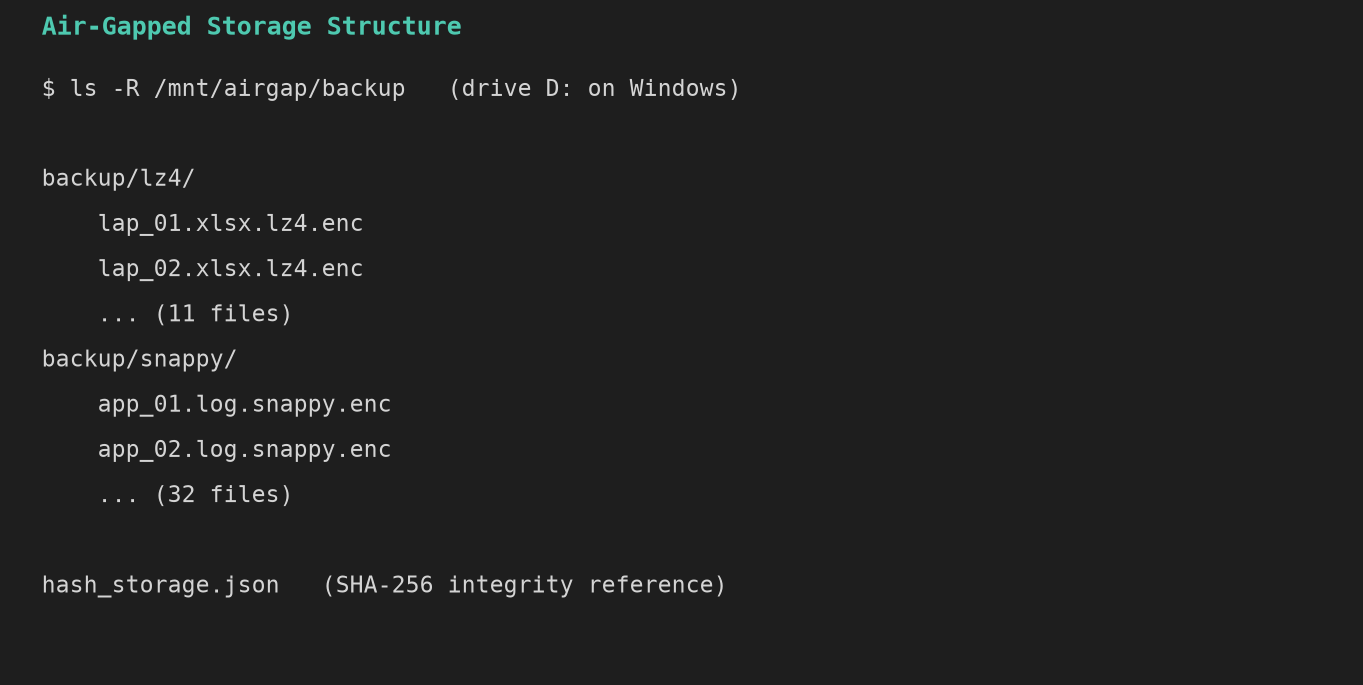
\includegraphics[width=0.85\textwidth]{figures/figure11_airgap_struct_en.png}
\vspace{.7em}
\caption{Air-gapped online storage}
\label{fig:airgap_storage}
\end{figure}

The air-gapped storage structure is shown in Figure~\ref{fig:airgap_storage}, where backup data is organized based on the compression algorithm used. In addition, the system stores hash-storage files in JavaScript Object Notation (JSON) format containing SHA-256 hash values of the original files and backup files as references for data integrity validation. This approach ensures that data integrity is maintained even when backups are stored on isolated media.

\subsection{Transfer and logging process to air-gapped storage}
The data transfer process to air-gapped storage is carried out in a controlled manner and automatically recorded in system logs. These logs record the reset and mounting stages of the storage media, followed by the data transfer process completed within a relatively short time.

\begin{figure}[H]
\centering
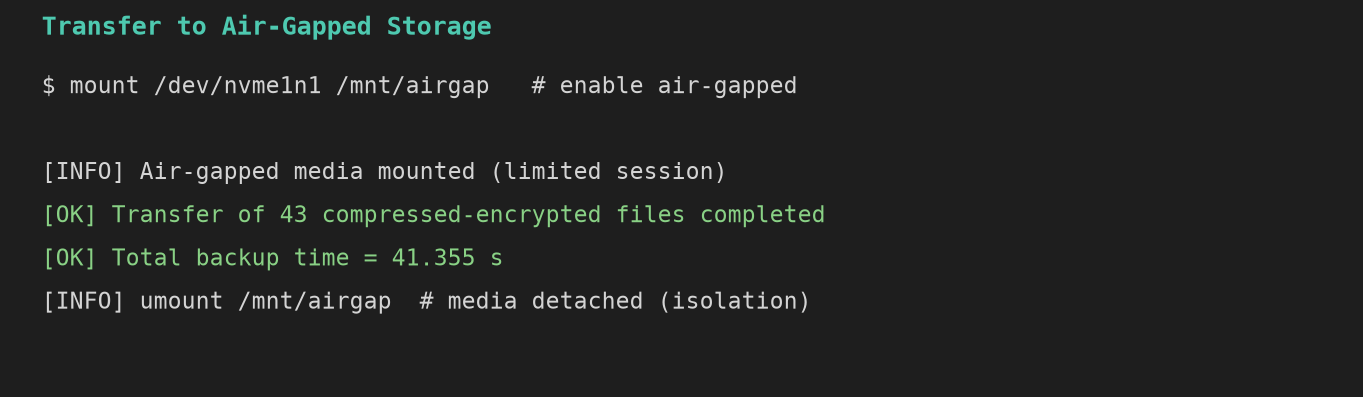
\includegraphics[width=\textwidth]{figures/figure12_transfer_en.png}
\vspace{.7em}
\caption{Transfer to air-gapped storage}
\label{fig:transfer}
\end{figure}

Figure~\ref{fig:transfer} displays information about the storage destination, processing time, and transfer success status. The existence of this logging mechanism allows the system to audit and trace backup activities in detail and serves as evidence that transfers to air-gapped media are performed separately and not continuously.

\subsection{System monitoring and data integrity validation}
System monitoring during the simulation is presented through an interactive dashboard shown in Figure~\ref{fig:dashboard}. This dashboard provides a summary of file status, compression ratios, compression time, validation results, and restore status for each compression algorithm used. This information is used to monitor system performance and conditions in real time.

\begin{figure}[H]
\centering
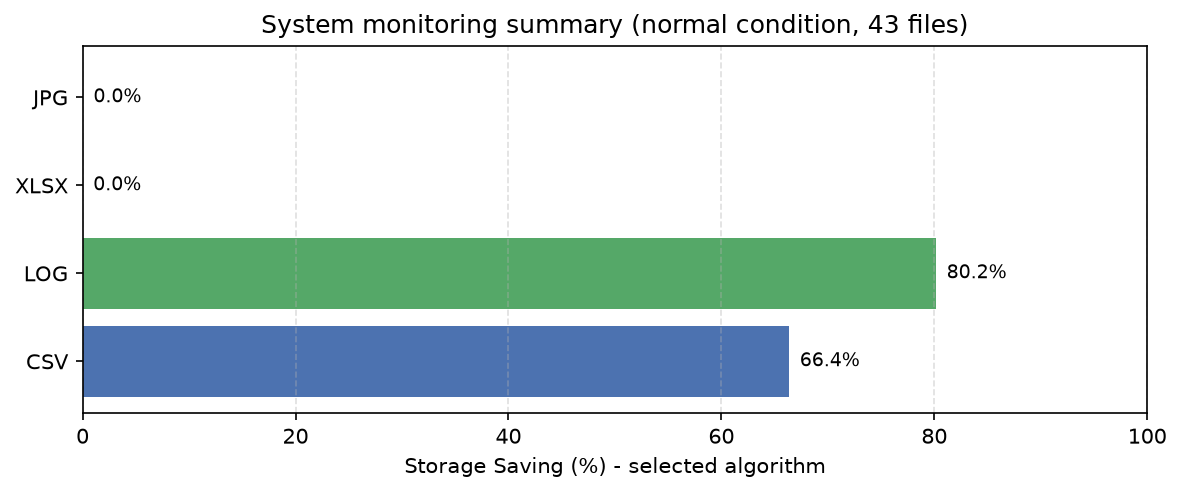
\includegraphics[width=\textwidth]{figures/figure13_dashboard_en.png}
\vspace{.7em}
\caption{System monitoring dashboard under normal conditions (no attack)}
\label{fig:dashboard}
\end{figure}

During the simulation, the system detected no anomalies in file structure or metadata. The checks include file size, file format/extension, and last modified timestamp. Additionally, the matching SHA-256 hash values confirm that no content changes or structural corruption occurred during the backup process.

\subsection{System simulation results under disrupted conditions (with ransomware attack)}
Testing under disrupted conditions was conducted to evaluate the system's ability to detect file changes caused by simulated ransomware attacks and to ensure backup availability in air-gapped storage. In this scenario, files in the main system were corrupted due to simulated attacks, while backup data remained secure in isolated air-gapped storage. When anomalies were detected through changes in hash values and metadata, the system automatically referred to backup copies for data recovery.

\subsubsection{File damage simulation results}
To evaluate system resilience, simulations were conducted on small to medium-sized files. Three types of damage were tested: Encrypt-and-hold, Metadata/Header Corruption, and Overwrite-and-corrupt. The results show that the backup mechanism can either maintain data integrity or enable recovery using air-gapped backups, even when original file content experiences partial or total damage.

\begin{table}[H]
\centering
\fontsize{8pt}{10pt}\selectfont
\caption{Results of file damage simulation due to ransomware attacks}
\label{tab:damage_simulation}
\begin{tabularx}{\textwidth}{@{}>{\raggedright\arraybackslash}p{2.2cm} >{\raggedright\arraybackslash}p{1.9cm} >{\raggedright\arraybackslash}X >{\raggedright\arraybackslash}X >{\raggedright\arraybackslash}X@{}}
\hline
\textbf{Attack Type} & \textbf{File Target} & \textbf{Simulation Method} & \textbf{Scenario Observation} & \textbf{Result} \\
\hline
Encrypt and Hold (CVE-2017-0144) & finance\_\-log\_\-500kb.log & Controlled modification of file content to simulate WannaCry ransomware encryption patterns & File changes to WNCRY format, with timestamp modified to 11/12/2025 09:58 & Files become unreadable, and the hash value differs from the original \\
Metadata/Header Corruption (CVE-2018-8453) & finance\_\-log\_\-500kb.log & Controlled modification of file headers & The initial part of the file is corrupted with random characters, while the lower part still displays valid log entries & The initial part of the file is corrupted, while the lower part still displays valid log entries \\
Overwrite-and-Corrupt (CVE-2021-36934) & finance\_\-log\_\-500kb.log & Controlled overwriting of partial file content with random characters & The log structure becomes disorganized; some INFO/ERROR/DEBUG patterns remain visible, and non-ASCII characters appear & Files cannot be recovered, and the hash value differs \\
Recovery Validation & finance\_\-log\_\-500kb.log & Restoration from air-gapped backup performed & --- & Original file successfully recovered \\
\hline
\end{tabularx}
\end{table}

Based on Table~\ref{tab:damage_simulation}, each attack type has a different impact on file structure and integrity. Encrypt-and-hold causes complete content modification, including increased file size and timestamp changes, making the file unreadable. Metadata/Header corruption affects the file's initial structure, allowing partial readability but compromising overall integrity. Overwrite-and-corrupt replaces parts of the file with random characters, producing disorganized structures with non-ASCII characters, making recovery impossible.

\subsubsection{Hash and metadata change analysis}
Further analysis was conducted to evaluate changes in hash values and file metadata before and after the ransomware attack simulation. This stage aims to assess the effectiveness of hash-based integrity checking mechanisms in detecting file modifications, whether partial or complete. The test results show that all files subjected to simulated attacks produced SHA-256 hash values that differ from their initial values before the attack. Hash changes occurred across all three damage scenarios: Encrypt and Hold, Metadata/Header Corruption, and Overwrite and Corrupt. These findings confirm that hash-based integrity checking is capable of accurately detecting file content changes, even when the damage occurs only in part of the file structure. In addition to hash values, several file metadata attributes also experienced significant changes.

\begin{table}[H]
\centering
\fontsize{8pt}{10pt}\selectfont
\caption{Hash and metadata changes of file before simulation}
\label{tab:hash_before}
\begin{tabularx}{\textwidth}{@{}X c c c@{}}
\hline
\textbf{File} & \textbf{SHA-256 Hash} & \textbf{File Size} & \textbf{Last Modified / MIME Type} \\
\hline
finance\_log\_500KB.log & cd5bda6156e87c84971e9a5e3500d521 & 500 KB & 2025-12-04 10:08:36 (UTC) / text/plain \\
\hline
\end{tabularx}
\end{table}

Table~\ref{tab:hash_before} shows the hash values and metadata of the test file before the ransomware simulation as a data integrity baseline. This hash value represents the initial condition of the file in a normal, readable state with no modifications. This baseline serves as the primary reference for comparing changes in hash and metadata after the ransomware attack simulation is performed.

\begin{table}[H]
\centering
\fontsize{8pt}{10pt}\selectfont
\caption{Hash and metadata changes of file after simulation}
\label{tab:hash_after}
\begin{tabularx}{\textwidth}{@{}p{2.3cm} >{\raggedright\arraybackslash}X c >{\raggedright\arraybackslash}p{2.2cm} >{\raggedright\arraybackslash}X@{}}
\hline
\textbf{Attack Type} & \textbf{SHA-256 Hash (truncated)} & \textbf{File Size} & \textbf{Last Modified} & \textbf{Status / Description} \\
\hline
Encrypt and Hold (CVE-2017-0144) & \texttt{2eb4e7bd18f290\-b66150a0d0d49\-bd79c} & 667 KB & 2026-01-06 20:56:49 & Changed; suspicious extension (MIME text/plain) \\
Metadata/Header Corruption (CVE-2018-8453) & \texttt{102453959e6585\-3e9257b095b9\-fcc27d048906} & 501 KB & 2026-01-14 20:22:08 & Changed; SHA-256 mismatch, file may be encrypted (MIME text/plain) \\
Overwrite-and-Corrupt (CVE-2021-36934) & \texttt{fc5f9e8b9c532f\-94acefedfdd7\-b11a91707634} & 501 KB & 2026-01-17 09:02:37 & Changed; SHA-256 mismatch, file may be encrypted (MIME text/plain) \\
\hline
\end{tabularx}
\end{table}

\subsubsection{System response to corrupted files}
The system automatically detects corrupted files during the recovery process by comparing checksums before and after recovery. If the checksum values do not match, the system marks the file as failed and activates \textit{air-gapped} recovery mode. In this mode, the system restores all files from an isolated backup repository to maintain data integrity. Recovery status and statistics are sent to the user interface in JSON format and displayed through visual notifications on the \textit{dashboard}. An example JSON output when \textit{air-gapped} mode is active shows \texttt{restore\_mode} set to \{mode: "airgap", reason: "ransomware\_detected", scope: "all"\}, \texttt{airgap} detected as true, a total restore of 43 files, a total restore OK of 43 files, and zero errors.

On the \textit{frontend} side, the interface displays clear visual notifications to the user. When \textit{air-gapped} mode is detected, the user receives a warning indicating that the system is performing a FULL RESTORE from the isolated backup, along with the number of successfully recovered files.

\begin{figure}[H]
\centering
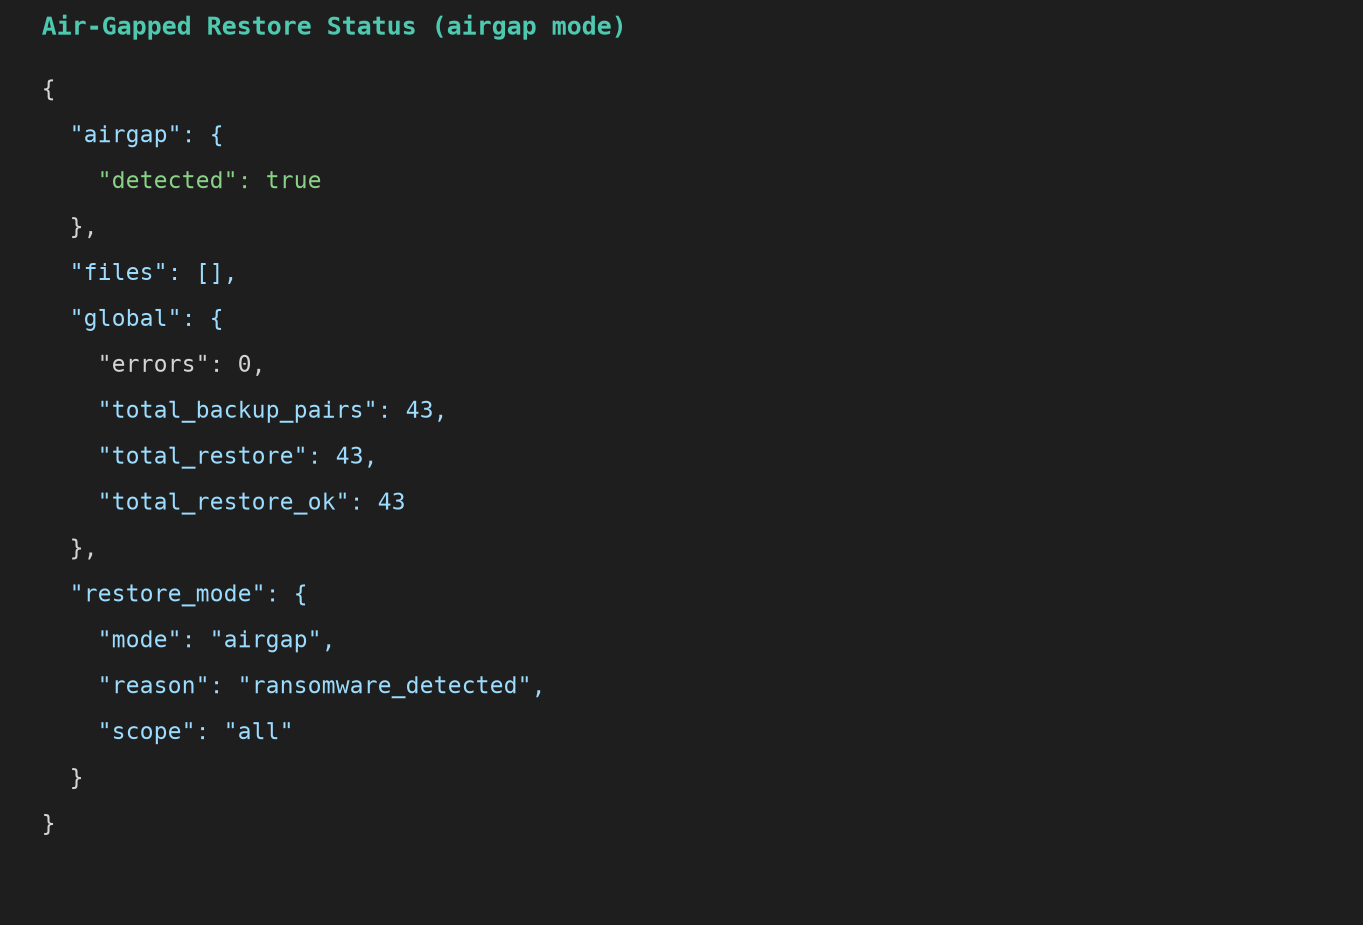
\includegraphics[width=0.8\textwidth]{figures/figure14_restore_json_en.png}
\vspace{.7em}
\caption{User interface showing restore status in air-gapped mode}
\label{fig:ui_restore}
\end{figure}

This approach ensures that corrupted files do not affect overall data integrity, and users can monitor recovery status in real time through an informative interface. With this method, the system proves resilient against corrupted files and capable of maintaining data security automatically through the \textit{air-gapped} recovery mode.

\subsection{Restore process from air-gapped backup}
After the system activates \textit{air-gapped} recovery mode, the data recovery process is carried out using backups stored on physically and logically isolated media. In this implementation, the \textit{air-gapped} mechanism is realized using a separate storage medium (Disk G:) dedicated exclusively as an isolated backup repository. This medium is not used for normal system operations and is only accessed during data recovery.

\begin{figure}[H]
\centering
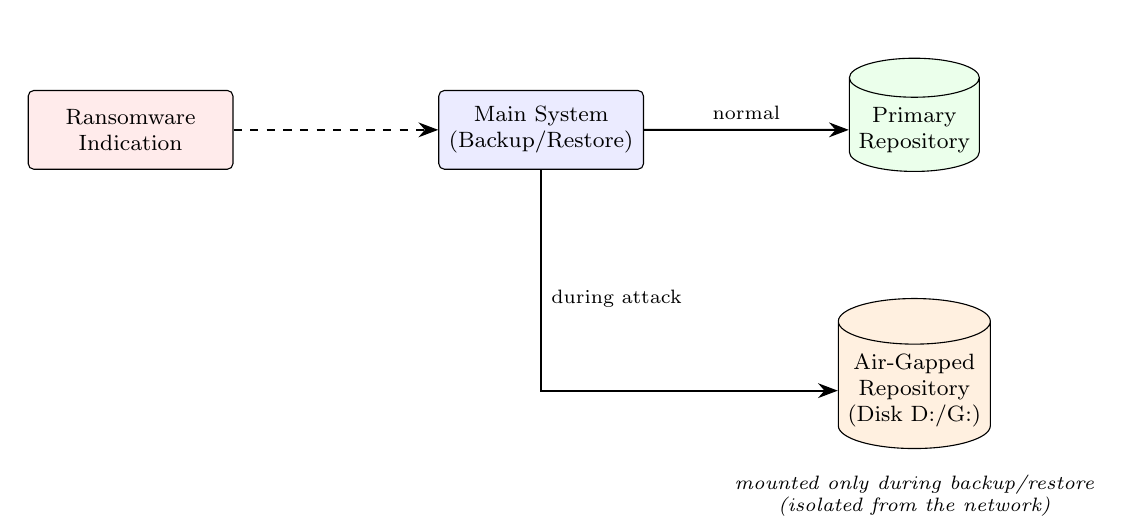
\begin{tikzpicture}[
    font=\footnotesize,
    box/.style={draw, rounded corners=2pt, minimum width=2.6cm, minimum height=1cm, align=center},
    store/.style={draw, cylinder, shape border rotate=90, aspect=0.3, minimum width=1.6cm, minimum height=1.4cm, align=center},
    ar/.style={-{Stealth[length=2.5mm]}, thick},
    ard/.style={-{Stealth[length=2.5mm]}, thick, dashed}
]
\node[box, fill=blue!8] (sys) {Main System\\(Backup/Restore)};
\node[store, right=2.6cm of sys, fill=green!8] (primary) {Primary\\Repository};
\node[store, below=1.6cm of primary, fill=orange!12] (airgap) {Air-Gapped\\Repository\\(Disk D:/G:)};
\node[box, left=2.6cm of sys, fill=red!8] (att) {Ransomware\\Indication};
% normal
\draw[ar] (sys) -- node[above]{\scriptsize normal} (primary);
% during attack -> switch to air-gapped
\draw[ard] (att) -- (sys);
\draw[ar] (sys.south) |- node[below right, font=\scriptsize, pos=0.25]{\scriptsize during attack} (airgap.west);
% isolation
\node[align=center, below=0.2cm of airgap, font=\scriptsize\itshape] {mounted only during backup/restore\\(isolated from the network)};
\end{tikzpicture}
\vspace{.7em}
\caption{VHDX media-based air-gapped backup architecture with network separation}
\label{fig:vhdx}
\end{figure}

Figure~\ref{fig:vhdx} illustrates the system architecture for data recovery using an air-gapped backup mechanism. Under normal conditions, the system performs backup and restore using the primary backup repository connected directly to the system. However, when critical conditions such as file corruption or ransomware attack indications are detected, the restore mechanism is switched to the air-gapped repository. This repository is implemented using a separate storage medium (Disk G:) that is physically and logically isolated from both the main system and the network.

\subsection{Decompression, decryption, data integrity validation, and recovery time evaluation}
Data integrity validation is performed after the recovery process to ensure that the recovered files are identical to the original data before the attack. Files recovered from the \textit{air-gapped} medium are in compressed-and-encrypted form, so the system first performs decryption using the AES-256 algorithm and the corresponding secret key, followed by decompression to return the file to its original form. After decryption, the system compares the SHA-256 \textit{checksum} value of the file before recovery (sha\_in) and after recovery (sha\_out). A file is considered valid if both \textit{checksum} values are identical, indicating that data integrity has been preserved throughout the backup and recovery process.

\begin{figure}[H]
\centering
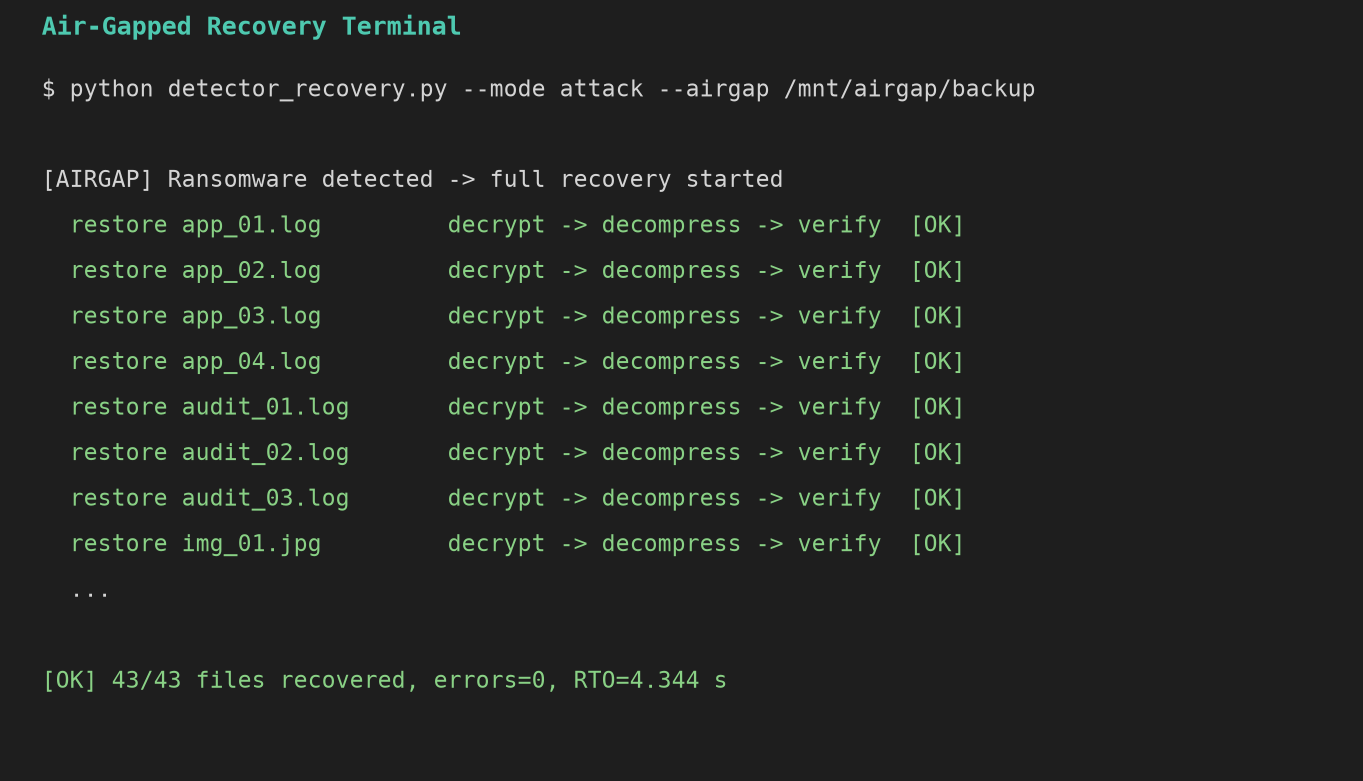
\includegraphics[width=\textwidth]{figures/figure16_restore_terminal_en.png}
\vspace{.7em}
\caption{Air-gapped restore process terminal showing the recovery and checksum validation of all files}
\label{fig:restore_terminal}
\end{figure}

The terminal results in Figure~\ref{fig:restore_terminal} show that all files were successfully recovered with status [OK], indicating that the recovery, decompression, decryption, and \textit{checksum} validation processes were successfully completed. Overall, the system successfully recovered 43 files without errors.

Recovery performance is evaluated using the \textit{Recovery Time Objective} (RTO), defined as the time required for the system to recover all 43 files from \textit{air-gapped} storage after an anomaly is detected. Testing was conducted on the EC2 (AWS) environment with a total dataset of $\approx 490$ MB. Table~\ref{tab:rto} presents the measured RTO for the three attack scenarios. The entire recovery process (AES-256 decryption, decompression, restoration, and SHA-256 re-verification) successfully returned 43 of 43 files without error in each scenario.

\begin{table}[H]
\centering
\fontsize{8pt}{10pt}\selectfont
\caption{Measured Recovery Time Objective (RTO) for recovering all 43 files}
\label{tab:rto}
\begin{tabular}{l c c c}
\hline
\textbf{Attack Type} & \textbf{Total Files} & \textbf{Files Recovered} & \textbf{RTO (seconds)} \\
\hline
Encrypt-and-Hold (CVE-2017-0144)        & 43 & 43 & 4.34 \\
Metadata/Header Corruption (CVE-2018-8453) & 43 & 43 & 5.21 \\
Overwrite-and-Corrupt (CVE-2021-36934)  & 43 & 43 & 5.34 \\
\hline
\end{tabular}
\end{table}

The measured RTO is in the range of 4.3--5.3 seconds to recover the entire test dataset. Because the recovery workflow is deterministic and its time increases approximately linearly with data volume, the RTO for larger enterprise-scale \textit{datasets} can be extrapolated proportionally; validation at full scale (files up to 1 GB) is part of future work.

\subsection{Cross-platform consistency of results (Windows vs Linux)}
The same experiment was run on AWS EC2 Windows Server 2022 and Ubuntu 22.04 instances to verify cross-platform consistency. Table~\ref{tab:cross_platform} compares the key results of the two environments. The compression ratios are practically identical on both platforms---because they depend on data and algorithm characteristics, not the operating system---while the only difference appears in recovery time (RTO) due to hardware differences. Detection and recovery reliability are both perfect (detection 43/43, recovery 43/43, FPR/FNR 0\%) on both platforms.

\begin{table}[H]
\centering
\fontsize{8pt}{10pt}\selectfont
\caption{Consistency of results across two platforms (43 files)}
\label{tab:cross_platform}
\begin{tabular}{l c c}
\hline
\textbf{Metric} & \textbf{Windows Server 2022} & \textbf{Ubuntu 22.04} \\
\hline
Log/TXT saving (Brotli) & 89.6\% & 89.5\% \\
CSV saving (Brotli)     & 81.1\% & 81.1\% \\
JPG / XLSX saving       & $\approx$0\% & $\approx$0\% \\
Detection (all attacks) & 43/43 & 43/43 \\
Successful recovery     & 43/43 & 43/43 \\
FPR / FNR               & 0\% / 0\% & 0\% / 0\% \\
RTO Encrypt-and-Hold (seconds) & 5.50 & 4.34 \\
RTO Metadata Corruption (seconds) & 5.20 & 5.21 \\
RTO Overwrite-and-Corrupt (seconds) & 5.32 & 5.34 \\
\hline
\end{tabular}
\end{table}

This agreement of results confirms that the proposed mechanisms---adaptive compression, integrity verification, and \textit{air-gapped} recovery---work reliably and reproducibly on both the local Windows environment and the Linux/Windows \textit{cloud} infrastructure, strengthening the external validity of the findings.

\subsection{False positive and false negative evaluation}
To evaluate the reliability of the ransomware detection mechanism, additional testing was conducted to measure the \textit{False Positive Rate} (FPR) and \textit{False Negative Rate} (FNR). The evaluation compared legitimate AES-256 backup encryption processes with simulated ransomware attacks that intentionally modified file content and metadata. When abnormal modifications were detected, the system automatically activated \textit{air-gapped} recovery mode and replaced corrupted files using isolated backup copies. This mechanism ensures that compromised files cannot continue to propagate within the system.

\begin{table}[H]
\centering
\fontsize{8pt}{10pt}\selectfont
\caption{Detection and recovery accuracy evaluation}
\label{tab:detection_accuracy}
\begin{tabularx}{\textwidth}{@{}X c c c c c@{}}
\hline
\textbf{Scenario} & \textbf{Total Files} & \textbf{Detected as Ransomware} & \textbf{Automatic Air-Gapped Restore} & \textbf{Actual Status} & \textbf{Result} \\
\hline
Normal AES-256 backup encryption & 43 & 0 & No & Safe & True Negative \\
Encrypt and Hold attack & 43 & 43 & Yes & Ransomware & True Positive \\
Metadata/Header Corruption & 43 & 43 & Yes & Ransomware & True Positive \\
Overwrite and Corrupt & 43 & 43 & Yes & Ransomware & True Positive \\
\hline
\end{tabularx}
\end{table}

Based on the experimental results, the \textit{False Positive Rate} (FPR) = 0\% and the \textit{False Negative Rate} (FNR) = 0\%. The results indicate that the system successfully distinguishes legitimate AES-256 encryption generated during normal backup operations from unauthorized file modifications caused by ransomware simulations. Furthermore, once anomalies are detected, the system automatically activates \textit{air-gapped} recovery mode to restore clean backup versions. This combination of integrity validation and isolated recovery improves both ransomware detection reliability and system resilience.

It must be emphasized that these FPR and FNR values of 0\% are a \textit{logical consequence} of the \textit{hash}-integrity-based detection mechanism in a controlled test environment, and are \textbf{not} a claim that the system will achieve perfect detection in a real-world operational environment. Because every file modification---even a single \textit{byte}---will deterministically change the SHA-256 \textit{hash} value, all simulated file corruption is necessarily detected, while legitimate backup encryption is never falsely flagged because its integrity baseline is recorded beforehand. In other words, this perfect result reflects the deterministic nature of \textit{hash} verification, not a capacity to generalize to real ransomware. In practice, integrity-based mechanisms like this have a fundamental limitation: they detect \textit{that} a file has changed, but do not analyze the \textit{behavior} of a process, making them vulnerable to sophisticated \textit{evasion} techniques such as \textit{Format-Preserving Encryption} (FPE), \textit{fileless ransomware}, and \textit{Living-off-the-Land} (LotL) that are not represented in the synthetic \textit{dataset} and controlled scenarios of this study. Therefore, the FPR/FNR figures above should be interpreted as functional validation at the mitigation and recovery stage, not as a benchmark for ransomware detection accuracy in general.

\subsection{Evaluation of system capability in distinguishing normal encryption and ransomware}
This evaluation aims to distinguish normal encryption in the backup mechanism from file changes caused by the ransomware simulation. In the normal backup process, the system records \textit{hash} values and metadata as an integrity baseline after controlled encryption and compression. In contrast, the ransomware simulation introduces significant deviations in \textit{hash} values and file structure that do not match the baseline. These differences are detected by the integrity validation mechanism, allowing compromised files to be identified. The results show that the combination of \textit{hash} checking, metadata analysis, and \textit{air-gapped} backup mechanisms effectively maintains data integrity while enabling secure recovery during ransomware attacks.

\subsection{Security analysis of the logical air-gap and window of vulnerability}
Unlike a physical \textit{air-gap} that fully severs the connection, the logical \textit{air-gap} approach adopted in this study isolates the backup volume by mounting it only during an active backup or recovery window. This model is more affordable and practical, but it must be honestly acknowledged that it leaves a \textit{window of vulnerability}: while the volume is mounted, it can technically be reached by other processes on the \textit{host}. Sophisticated, \textit{memory-resident} ransomware could potentially wait for a \textit{mount} event and then immediately write a malicious payload to the backup media. Thus, logical isolation substantially reduces the attack surface compared with a continuously connected repository, but does not eliminate it entirely.

To narrow this window, several mitigations can be applied and are recommended as part of a practical deployment. First, strict access-privilege restriction through \textit{Identity and Access Management} (IAM) so that only authorized backup processes may trigger a \textit{mount} and write to the volume. Second, applying read-only (\textit{read-only}) \textit{mount} mode during recovery operations, so the restoration process cannot be exploited to write a malicious payload. Third, the use of \textit{immutable}/WORM (\textit{write-once-read-many}) storage, for example through an \textit{object lock} on cloud object storage, so that backup versions that have been written cannot be altered or deleted during the retention period. Fourth, minimizing the \textit{mount} duration as tightly as possible---only for the duration of the backup transaction---to reduce the opportunity for exploitation. This combination of controls makes the logical \textit{air-gap} a reasonable compromise among cost, operational ease, and resilience, while opening a direction for strengthening toward a \textit{zero-trust backup} architecture in future work.

\section{Conclusion}
\label{sec:conclusion}
A cloud-based backup system integrating an \textit{air-gapped} backup mechanism with multi-algorithm \textit{lossless} compression was developed to improve resilience against ransomware attacks while optimizing storage efficiency. The system successfully performs compression, backup, anomaly detection, and automated data recovery within an integrated environment. Experimental results demonstrate that compression performance depends on data characteristics. Snappy and LZ4 provide faster processing times for small and medium-sized files, while Brotli and Zstandard achieve the highest compression ratios on low-entropy text files, with storage savings of up to 89.5\% for log files and 81.1\% for CSV files; already-compressed files (JPG, XLSX) show savings close to zero, in line with the theoretical limit of \textit{lossless} compression.

Controlled ransomware simulations (without real \textit{malware}) on a synthetic \textit{dataset} of 43 files, using several attack scenarios based on the CVE-2017-0144, CVE-2018-8453, and CVE-2021-36934 patterns, demonstrated that the proposed system successfully maintained data integrity and achieved a 100\% data recovery rate across all 43 tested files through the \textit{air-gapped} backup mechanism. In addition, the anomaly detection mechanism successfully detected unauthorized file modifications while maintaining zero \textit{false positives} during normal AES-256 encryption operations. These findings indicate that integrating an \textit{air-gapped} backup architecture with multi-algorithm compression significantly enhances both system resilience and storage efficiency in cloud-based backup environments.

The adaptive compression mechanism currently uses a rule-based selection strategy because of its lower computational \textit{overhead}, lightweight implementation, and faster decision-making capability for cloud backup environments that require efficient resource utilization and rapid recovery response. This approach is considered suitable for financial cloud systems where reliability and low-latency operation are critical.

This study has several limitations that in turn open directions for future research. First, validation was carried out on a limited-size synthetic \textit{dataset} (43 files) through controlled simulation, so generalization to large-scale enterprise workloads and to real ransomware behavior still needs to be tested. Second, the detection mechanism relies on \textit{hash} and metadata integrity and therefore does not yet handle sophisticated evasion. Several promising directions for development include: (i) refining the rule-based compression algorithm selection into a \textit{machine learning}-based one (e.g., \textit{Random Forest}) to improve accuracy and scalability on larger and more heterogeneous data; (ii) testing with real ransomware samples in a safe \textit{sandbox} environment; (iii) integrating \textit{immutable}/WORM backup storage and a \textit{zero-trust backup} architecture; (iv) formal security analysis and stronger \textit{key management}; (v) evaluation at enterprise scale with measurements of \textit{throughput}, CPU/RAM utilization, energy consumption, and \textit{cloud} cost; and (vi) direct comparison with other backup strategies such as \textit{incremental backup} and \textit{deduplication}. These directions are expected to strengthen the credibility, resilience, and practical feasibility of the ransomware-resilient backup system.

\section*{FUNDING INFORMATION}
\label{sec:funding}
This research was supported by Politeknik Elektronika Negeri Surabaya and conducted in collaboration with PT Equnix Business Solution with support from internal resources.

\section*{AUTHOR CONTRIBUTIONS STATEMENT}
\label{sec:credit}
This study employs the Contributor Roles Taxonomy (CRediT) to acknowledge individual author contributions, mitigate authorship conflicts, and enhance collaboration.

\begin{table}[H]
	\centering
	\selectfont
	\begin{tabular}{lcccccccccccccc}
		\hline
		\textbf{Name of Author} & \cellcolor[HTML]{D8F0F8}\textbf{C} & \cellcolor[HTML]{D8F0F8}\textbf{M} & \textbf{So} & \textbf{Va} & \cellcolor[HTML]{D8F0F8}\textbf{Fo} & \cellcolor[HTML]{D8F0F8}\textbf{I} & \textbf{R} & \textbf{D} & \cellcolor[HTML]{FDE9D9}\textbf{O} & \cellcolor[HTML]{FDE9D9}\textbf{E} & \textbf{Vi} & \textbf{Su} & \textbf{P} & \textbf{Fu} \\
		\hline
		Hero Yudo Martono & \cellcolor[HTML]{D8F0F8}\checkmark & \cellcolor[HTML]{D8F0F8}\checkmark & \checkmark & \checkmark & \cellcolor[HTML]{D8F0F8}\checkmark & \cellcolor[HTML]{D8F0F8}\checkmark &  & \checkmark & \cellcolor[HTML]{FDE9D9}\checkmark & \cellcolor[HTML]{FDE9D9}\checkmark &  & \checkmark & \checkmark & \checkmark \\
		Nafisah Rahmadani H. & \cellcolor[HTML]{D8F0F8} & \cellcolor[HTML]{D8F0F8}\checkmark & \checkmark &  & \cellcolor[HTML]{D8F0F8}\checkmark & \cellcolor[HTML]{D8F0F8}\checkmark & \checkmark & \checkmark & \cellcolor[HTML]{FDE9D9}\checkmark & \cellcolor[HTML]{FDE9D9} & \checkmark &  &  &  \\
		Iwan Syarif & \cellcolor[HTML]{D8F0F8}\checkmark & \cellcolor[HTML]{D8F0F8}\checkmark &  & \checkmark & \cellcolor[HTML]{D8F0F8} & \cellcolor[HTML]{D8F0F8} &  &  & \cellcolor[HTML]{FDE9D9} & \cellcolor[HTML]{FDE9D9}\checkmark &  & \checkmark &  &  \\
		Ferry Astika Saputra & \cellcolor[HTML]{D8F0F8}\checkmark & \cellcolor[HTML]{D8F0F8}\checkmark &  & \checkmark & \cellcolor[HTML]{D8F0F8} & \cellcolor[HTML]{D8F0F8} &  &  & \cellcolor[HTML]{FDE9D9} & \cellcolor[HTML]{FDE9D9}\checkmark &  & \checkmark &  &  \\
		\hline
		\multicolumn{15}{c}{
			\begin{tabular}{llllll}
				&&&&&\\
				C &: 	\textbf{C}\fontsize{8}{10}\selectfont onceptualization \quad\quad\quad\quad\quad\quad& I &: 	\textbf{I}\fontsize{8}{10}\selectfont nvestigation & Vi&: 	\textbf{Vi}\fontsize{8}{10}\selectfont sualization  \\
				M &: 	\textbf{M}\fontsize{8}{10}\selectfont ethodology & R &: 	\textbf{R}\fontsize{8}{10}\selectfont esources & Su&: 	\textbf{Su}\fontsize{8}{10}\selectfont pervision  \\
				So&: 	\textbf{So}\fontsize{8}{10}\selectfont ftware & D &:	\textbf{D}\fontsize{8}{10}\selectfont ata Curation & P &: 	\textbf{P}\fontsize{8}{10}\selectfont roject Administration  \\
				Va&: 	\textbf{Va}\fontsize{8}{10}\selectfont lidation & O &:	\fontsize{8}{10}\selectfont Writing - \fontsize{10}{12}\selectfont \textbf{O}\fontsize{8}{10}\selectfont riginal Draft & Fu&: 	\textbf{Fu}\fontsize{8}{10}\selectfont nding Acquisition \\
				Fo&: 	\textbf{Fo}\fontsize{8}{10}\selectfont rmal Analysis & E &:	\fontsize{8}{10}\selectfont Writing - Review \& \fontsize{10}{12}\selectfont\textbf{E}\fontsize{8}{10}\selectfont diting \quad\quad\quad\quad\quad\quad&  \\
			\end{tabular}
		}
	\end{tabular}
\end{table}

\section*{CONFLICT OF INTEREST STATEMENT}
\label{sec:coi}
The authors declare that there is no conflict of interest regarding the publication of this paper.

\section*{DATA AVAILABILITY}
\label{sec:data}
Datasets used in this study were synthetically generated based on operational data characteristics and backup structures adapted from PT Equnix Business Solution environments. No real financial or confidential production data were used in this study.

\section*{REFERENCES}
\label{sec:references}
\footnotesize

\begin{thebibliography}{99}
\footnotesize
\itemsep 0pt

\bibitem{1} A. A. Majmuah, ``Survey on technique to prevent ransomware attack,'' \textsl{Bulletin of Informatics and Data Science}, vol. 1, no. 2, 2021.
\bibitem{2} K. Begovi\'c, M. Karabegovi\'c, and A. Huseinovi\'c, ``Cryptographic ransomware encryption detection: survey,'' \textsl{arXiv preprint arXiv:2306.12008}, 2023.
\bibitem{3} S. Mansfield-Devine, ``Ransomware: detection, prevention and cure,'' \textsl{Network Security}, vol. 2016, no. 9, pp. 5--8, 2016.
\bibitem{4} H. B. Pavlos, P. Nikolaos, A. Jawad, and J. William, ``Ransomware: analysing the impact on Windows Active Directory Domain Services,'' \textsl{Journal of Cyber Security Technology}, 2022.
\bibitem{5} M. Houria, O. Noura, and A. Abdelmalek, ``Ransomware: analysis of encrypted files,'' \textsl{International Journal of Information Security}, 2023.
\bibitem{6} G. Lu, Y. Liu, Y. Chen, C. Zhang, Y. Gao, and G. Zhong, ``A comprehensive detection approach of WannaCry: principles, rules and experiments,'' in \textsl{Proc. Int. Conf. Cyber-Enabled Distributed Computing and Knowledge Discovery (CyberC)}, 2020, pp. 41--49.
\bibitem{7} I. Athauda and H. Herath, ``Windows elevation of privilege serious SAM vulnerability (CVE-2021-36934),'' \textsl{Journal of Cybersecurity and Digital Forensics}, 2022.
\bibitem{8} A. Al-Fuqaha et al., ``A survey on ransomware trends and mitigation techniques,'' \textsl{Egyptian Informatics Journal}, vol. 21, no. 4, pp. 231--245, 2020.
\bibitem{9} Z. A. Syed and T. R. Soomro, ``Compression algorithms: Brotli, Gzip and Zopfli perspective,'' \textsl{International Journal of Computer Science and Network Security}, 2021.
\bibitem{10} F. A. Abdulazeez, I. T. Ahmed, and B. T. Hammad, ``Performance comparison of compression algorithms for large-scale log systems,'' \textsl{Journal of Computer \& Electrical Engineering Sciences}, 2024.
\bibitem{11} M. A. Rabbani, A. Budiyono, and A. Widjajarto, ``Implementasi dan analisis security auditing menggunakan open source software dengan framework MITRE ATT\&CK,'' \textsl{e-Proceeding of Engineering}, vol. 7, no. 2, 2020.
\bibitem{12} R. Y. Dwiaranda, A. Budiyono, and A. Widjajarto, ``Implementasi dan analisis security auditing menggunakan open source software dengan framework STRIDE,'' \textsl{e-Proceeding of Engineering}, vol. 7, no. 2, 2020.
\bibitem{13} M. Sahu and J. Panda, ``Performance evaluation of efficient hybrid compression methods for text using lossless algorithms,'' \textsl{arXiv preprint}, 2025.
\bibitem{14} H. Zhang et al., ``Optimized Snappy compression with enhanced encoding strategies,'' \textsl{Electronics}, 2024.
\bibitem{15} M. C. Ghanem, T. M. Chen, M. A. Ferrag, and M. E. Kettouche, ``ESASCF: automated security compliance framework,'' \textsl{arXiv preprint}, 2023.
\bibitem{16} S. Rouhani, R. Belchior, R. S. Cruz, and R. Deters, ``Distributed attribute-based access control system using a permissioned blockchain,'' \textsl{arXiv preprint}, 2020.
\bibitem{17} Y. Fauzi and R. A. Hamdan, ``Pendekatan metodologis dalam deteksi ancaman siber pada server hosting menggunakan NMAP dan Metasploit,'' \textsl{Jurnal SUDO}, 2024.
\bibitem{18} T. Ariyadi et al., ``Implementasi OWASP untuk analisis kerentanan dan keamanan sistem informasi,'' \textsl{Jurnal STORAGE}, 2023.
\bibitem{19} Sophos, ``The state of ransomware in financial services 2024,'' Sophos Ltd., 2024. [Online]. Available: https://www.sophos.com
\bibitem{20} R. Pal, M. Shaikh, J. Sagvekar, and P. Tiwari, ``Data resilience: secure emergency backup on cloud,'' \textsl{International Journal of Advanced Research in Science, Communication and Technology}, vol. 4, no. 7, 2024.
\bibitem{21} NIST, ``Security guidelines for storage infrastructure (SP 800-209),'' National Institute of Standards and Technology, 2024. [Online]. Available: https://nvlpubs.nist.gov
\bibitem{22} A. Nasif, Z. A. Othman, and N. S. Sani, ``The deep learning solutions on lossless compression methods for alleviating data load on IoT nodes in smart cities,'' \textsl{Sensors}, vol. 21, no. 12, p. 4223, 2021.
\bibitem{23} T. McIntosh, T. Susnjak, T. Liu, D. Xu, P. Watters, D. Liu, Y. Hao, A. Ng, and M. Halgamuge, ``Ransomware reloaded: re-examining its trend, research and mitigation in the era of data exfiltration,'' \textsl{ACM Computing Surveys}, vol. 57, no. 1, art. 18, pp. 1--40, 2024, doi: 10.1145/3691340.
\bibitem{24} S. Liu, F. Saeed, Z. Yang, and J. Chen, ``A comprehensive review on hyperspectral image lossless compression algorithms,'' \textsl{Remote Sensing}, vol. 17, no. 24, p. 3966, 2025.
\bibitem{25} J. Hua, H. Xu, Y. Du, and L. Du, ``Improved JPEG lossless compression for compression of intermediate layers in neural networks based on compute-in-memory,'' \textsl{Electronics}, vol. 13, no. 19, p. 3872, 2024.
\bibitem{26} C. Beaman, A. Barkworth, T. D. Akande, S. Hakak, and M. K. Khan, ``Ransomware: recent advances, analysis, challenges and future research directions,'' \textsl{Computers \& Security}, vol. 111, p. 102490, 2021, doi: 10.1016/j.cose.2021.102490.
\bibitem{27} M. Dawood et al., ``Cyberattacks and security of cloud computing: a complete guideline,'' \textsl{Symmetry}, vol. 15, no. 11, p. 1981, 2023.
\bibitem{28} A. Singh et al., ``Enhancing ransomware attack detection using transfer learning and deep learning ensemble models on cloud-encrypted data,'' \textsl{Electronics}, vol. 12, no. 18, p. 3899, 2023.
\bibitem{29} P. Novak et al., ``Multistage malware detection method for backup systems,'' \textsl{Technologies}, vol. 12, no. 2, p. 23, 2024.
\bibitem{30} Kritika, ``A comprehensive literature review on ransomware detection using deep learning,'' \textsl{Cyber Security and Applications}, vol. 3, p. 100078, 2025, doi: 10.1016/j.csa.2024.100078.
\bibitem{31} N. Ebrahimi Majd and T. Mazumdar, ``Ransomware classification using machine learning,'' in \textsl{Proc. 32nd Int. Conf. Advanced Information Networking and Applications (AINA)}, IEEE, 2023.
\bibitem{32} S. Enomoto, H. Kuzuno, H. Yamada, Y. Shiraishi, and M. Morii, ``Early mitigation of CPU-optimized ransomware using monitoring encryption instructions,'' \textsl{International Journal of Information Security}, vol. 23, pp. 3393--3413, 2024, doi: 10.1007/s10207-024-00892-2.
\bibitem{33} M. Lang, L. Connolly, P. Taylor, and P. J. Connert, ``The evolving menace of ransomware: a comparative analysis of pre-pandemic and mid-pandemic attacks,'' \textsl{Digital Threats: Research and Practice}, vol. 4, no. 4, pp. 1--22, 2023, doi: 10.1145/3558006.
\bibitem{34} Z. Pan and Z. Shu, ``Hardware-assisted ransomware detection using automated machine learning,'' in \textsl{Proc. Design, Automation \& Test in Europe Conf. (DATE)}, IEEE, 2025.
\bibitem{35} Y. Hou, L. Guo, C. Zhou, Y. Xu, Z. Yin, S. Li, C. Sun, and Y. Jiang, ``An empirical study of data disruption by ransomware attacks,'' in \textsl{Proc. IEEE/ACM 46th Int. Conf. Software Engineering (ICSE)}, 2024, pp. 1--12.
\bibitem{36} M. Smith and J. Lee, ``Performance evaluation of compression algorithms for cloud storage,'' \textsl{Data in Brief}, vol. 48, pp. 1--10, 2023.
\bibitem{37} S. Kumar and R. Patel, ``Optimization of cloud backup against ransomware attacks,'' \textsl{IEEE Access}, vol. 10, pp. 45821--45835, 2022.
\bibitem{38} A. Novak, P. Chen, and R. Singh, ``Hybrid compression and air-gapped backup for ransomware mitigation,'' in \textsl{Proc. USENIX Security Symposium}, 2021.
\bibitem{39} L. Zhao and T. Wang, ``Text compression optimization using hybrid algorithms,'' \textsl{arXiv preprint arXiv:2501.12345}, 2025.
\bibitem{40} P. H. Meland, Y. F. F. Bayoumy, and G. Sindre, ``The ransomware-as-a-service economy within the darknet,'' \textsl{Computers \& Security}, vol. 92, p. 101762, 2020, doi: 10.1016/j.cose.2020.101762.
\bibitem{41} G. Nagar, ``The evolution of ransomware: tactics, techniques, and mitigation strategies,'' \textsl{SSRN Electronic Journal}, 2024, doi: 10.2139/ssrn.4881213.
\bibitem{42} A. Kapoor, A. Gupta, R. Gupta, S. Tanwar, G. Sharma, and I. E. Davidson, ``Ransomware detection, avoidance, and mitigation scheme: a review and future directions,'' \textsl{Sustainability}, vol. 14, no. 1, p. 8, 2022, doi: 10.3390/su14010008.
\bibitem{43} J. Lee, J. Kim, H. Jeong, and K. Lee, ``A machine learning-based ransomware detection method for attackers' neutralization techniques using format-preserving encryption,'' \textsl{Sensors}, vol. 25, no. 8, p. 2406, 2025, doi: 10.3390/s25082406.
\bibitem{44} J. Thomas and G. Galligher, ``Improving backup system evaluations in information security risk assessments to combat ransomware,'' \textsl{Computer and Information Science}, vol. 11, no. 1, pp. 25--38, 2018, doi: 10.5539/cis.v11n1p25.
\bibitem{45} B. Bahl and R. Endicott, ``Know thy ransomware response: a detailed framework for devising effective ransomware response strategies,'' \textsl{Digital Threats: Research and Practice}, vol. 4, no. 4, pp. 1--19, 2020, doi: 10.1145/3560022.
\bibitem{46} P. Yan and T. T. Khoei, ``Securing the Internet of Things: a comprehensive review of ransomware attacks, detection, countermeasures, and future prospects,'' \textsl{Franklin Open}, vol. 11, art. 102056, 2025, doi: 10.1016/j.fraope.2025.102056.

\end{thebibliography}

\section*{BIOGRAPHIES OF AUTHORS}
\label{sec:biographies}

\noindent
\begin{tabularx}{\textwidth}{@{}m{2.5cm}@{\hspace{0.4cm}}X@{}}
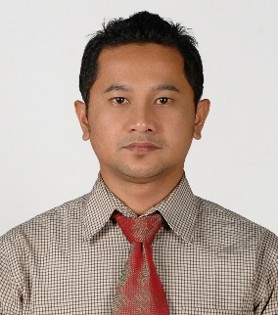
\includegraphics[width=2.5cm,height=3.2cm,keepaspectratio]{figures/hero.jpg} &
\textbf{Hero Yudo Martono} received his bachelor's degree in Computer Science (Electrical Engineering) from ITS, Indonesia. He then pursued a master's degree in Informatics Engineering from ITB, Indonesia. His research interests include cybersecurity, artificial intelligence, and cloud computing. He can be contacted at email: hero@pens.ac.id. \\
\end{tabularx}

\vspace{.7em}
\noindent
\begin{tabularx}{\textwidth}{@{}m{2.5cm}@{\hspace{0.4cm}}X@{}}
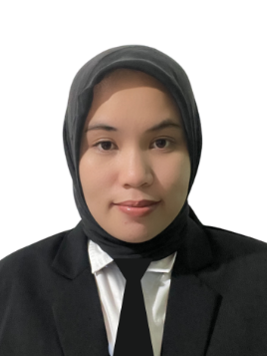
\includegraphics[width=2.5cm,height=3.2cm,keepaspectratio]{figures/nafisah.png} &
\textbf{Nafisah Rahmadani Harahap} is currently pursuing the Bachelor of Applied Engineering (D4) degree in Informatics Engineering at Politeknik Elektronika Negeri Surabaya (PENS), Indonesia. She is also working as an ERP Project Manager, focusing on enterprise resource planning implementation, business process optimization, project coordination, and digital transformation initiatives. Her research interests include cybersecurity, information systems, artificial intelligence, cloud computing, and enterprise software solutions. She can be contacted at email: nafisah@it.student.pens.ac.id. \\
\end{tabularx}

\vspace{.7em}
\noindent
\begin{tabularx}{\textwidth}{@{}m{2.5cm}@{\hspace{0.4cm}}X@{}}
\figplaceholder{2.5cm}{iwan.jpg} &
\textbf{Iwan Syarif} is a professor (Ph.D.) and lecturer at the Department of Informatics Engineering, Politeknik Elektronika Negeri Surabaya (PENS), Indonesia. His research focuses on cybersecurity. He can be contacted at email: iwanarif@pens.ac.id. \\
\end{tabularx}

\vspace{.7em}
\noindent
\begin{tabularx}{\textwidth}{@{}m{2.5cm}@{\hspace{0.4cm}}X@{}}
\figplaceholder{2.5cm}{ferry.jpg} &
\textbf{Ferry Astika Saputra} received his doctoral (Ph.D.) degree from Universitas Indonesia and is a lecturer at the Department of Informatics Engineering, Politeknik Elektronika Negeri Surabaya (PENS), Indonesia. His research focuses on cybersecurity. He can be contacted at email: ferryas@pens.ac.id. \\
\end{tabularx}

\end{document}
